\documentclass[a4paper,oneside,12pt]{book}

% Manuscrito v4. Reescrito desde cero sobre los resultados de octubre de 2026:
% corrida principal sin el periodo del cierre del mercado (pasos 1 a 42), etiquetas
% corregidas (modo C), tres semillas de modelo en todo. El manuscrito v3 (tesis_latex/)
% queda como registro histórico y sus cifras de Elliptic están retractadas.

\usepackage[utf8]{inputenc}
\usepackage[T1]{fontenc}
\usepackage[spanish,es-lcroman,es-tabla,es-nodecimaldot]{babel}
\usepackage[margin=1in]{geometry}

\usepackage{amsmath,amssymb,mathtools}
\usepackage{graphicx}
\graphicspath{{figuras/}}
\usepackage{float}
\usepackage{booktabs,tabularx,longtable}
\usepackage[table,xcdraw]{xcolor}
\usepackage{subcaption}
\usepackage{setspace}
\usepackage{caption}
\captionsetup{font=small,labelfont=bf,width=0.95\textwidth}

\usepackage{fancyhdr}
\pagestyle{fancy}
\fancyhf{}
\fancyhead[L]{\leftmark}
\fancyhead[R]{\thepage}
\renewcommand{\headrulewidth}{0.4pt}
\setlength{\headheight}{15.13202pt}
\addtolength{\topmargin}{-3.13202pt}

\usepackage{mathptmx}
\renewcommand{\ttdefault}{lmtt}

\setlength{\parindent}{0pt}
\setlength{\parskip}{6pt plus 2pt minus 1pt}
\setlength{\emergencystretch}{2em}
\onehalfspacing

% Los artículos (generados desde Crossref) solo traen DOI; las excepciones (actas y arXiv)
% traen la URL donde se verificaron.
\usepackage[backend=biber,style=numeric,sorting=none,doi=true,url=true,eprint=true,
            isbn=false,maxbibnames=6,minbibnames=3]{biblatex}
\addbibresource{bibliografia.bib}
\AtBeginBibliography{\sloppy\small}

\usepackage[hidelinks]{hyperref}
\urlstyle{same}

\newcommand{\pd}{p\text{-valor}}

\begin{document}

% ================================================= PORTADAS
\begin{titlepage}
\begin{center}

\includegraphics[width=0.4\textwidth]{utp.jpg}

\vspace{1.5cm}
{\LARGE \bfseries \linespread{1.3}\selectfont
Estabilidad de las explicaciones de redes neuronales de grafos para la detección de lavado
de dinero bajo desbalance extremo de clases\par}

\vspace{2.5cm}
{\Large Alejandro Gómez Huertas \\[0.3cm] Juan Diego Garzón Ovalle}

\vfill
{\large Universidad Tecnológica de Pereira \\ Facultad de Ingenierías \\
Maestría en Ingeniería de Sistemas y Computación \\ Pereira, Colombia \\ 2026}
\end{center}
\end{titlepage}

\begin{titlepage}
\begin{center}
\vspace*{1cm}
{\LARGE \bfseries \linespread{1.3}\selectfont
Estabilidad de las explicaciones de redes neuronales de grafos para la detección de lavado
de dinero bajo desbalance extremo de clases\par}

\vspace{2cm}
{\Large Alejandro Gómez Huertas \\[0.3cm] Juan Diego Garzón Ovalle}

\vspace{2.5cm}
{\large Tesis presentada como requisito parcial para optar al título de:}\\[0.5cm]
{\Large \textbf{Magíster en Ingeniería de Sistemas y Computación}}

\vspace{2cm}
{\large \textbf{Director} \\[0.2cm] \Large Ph.D. Cristian Rosero Arias}

\vfill
{\large Universidad Tecnológica de Pereira \\ Facultad de Ingenierías \\
Maestría en Ingeniería de Sistemas y Computación \\ Pereira, Colombia \\ 2026}
\end{center}
\end{titlepage}

\pagenumbering{roman}
\chapter*{Resumen}
\addcontentsline{toc}{chapter}{Resumen}
\textbf{[Por redactar al cerrar los Capítulos 5 a 7.]}

\vspace{0.4cm}
\noindent\textbf{Palabras clave:} redes neuronales de grafos, explicabilidad, estabilidad de
las explicaciones, lavado de dinero, desbalance de clases, Elliptic.

\chapter*{Abstract}
\addcontentsline{toc}{chapter}{Abstract}
\textbf{[To be written once Chapters 5 to 7 are closed.]}

\vspace{0.4cm}
\noindent\textbf{Keywords:} graph neural networks, explainability, explanation stability,
money laundering, class imbalance, Elliptic.


\clearpage
\tableofcontents
\clearpage
\listoffigures
\addcontentsline{toc}{chapter}{Índice de figuras}
\clearpage
\listoftables
\addcontentsline{toc}{chapter}{Índice de tablas}
\clearpage
\chapter*{Lista de acrónimos}
\addcontentsline{toc}{chapter}{Lista de acrónimos}
\begin{longtable}{p{0.19\textwidth}p{0.75\textwidth}}
\textbf{AML} & \textit{Anti-Money Laundering}, prevención del lavado de dinero \\[2pt]
\textbf{EG} & \textit{Expected Gradients} \\[2pt]
\textbf{F1} & Media armónica de precisión y exhaustividad \\[2pt]
\textbf{GAT} & \textit{Graph Attention Network}, red de grafos con atención \\[2pt]
\textbf{GCN} & \textit{Graph Convolutional Network}, red convolucional de grafos \\[2pt]
\textbf{GNN} & \textit{Graph Neural Network}, red neuronal de grafos \\[2pt]
\textbf{GraphSAGE} & \textit{Graph Sample and Aggregate} \\[2pt]
\textbf{IG} & \textit{Integrated Gradients} \\[2pt]
\textbf{MCC} & Coeficiente de correlación de Matthews \\[2pt]
\textbf{PR-AUC} & Área bajo la curva de precisión y exhaustividad \\[2pt]
\textbf{ROC-AUC} & Área bajo la curva ROC \\[2pt]
\textbf{SMOTE} & \textit{Synthetic Minority Over-sampling Technique} \\[2pt]
\textbf{TAGCN} & \textit{Topology Adaptive Graph Convolutional Network} \\[2pt]
\textbf{TOST} & \textit{Two One-Sided Tests}, prueba de equivalencia \\[2pt]
\textbf{XAI} & \textit{Explainable Artificial Intelligence}, inteligencia artificial explicable \\[2pt]
\end{longtable}


\clearpage
\pagenumbering{arabic}
\chapter{Introducción}\label{cap:introduccion}

\section{Planteamiento del problema}

La detección de lavado de dinero se apoya cada vez más en modelos de aprendizaje automático
que examinan transacciones en busca de patrones anómalos \cite{Chen2018AMLReview,
Kute2021AMLReview}. En el caso de las criptomonedas, las transacciones forman de manera natural
un grafo, en el que cada transacción es un nodo y cada transferencia de fondos entre
transacciones es una arista. Las redes neuronales de grafos (\textit{Graph Neural Networks},
GNN) aprovechan esa estructura combinando los atributos de cada transacción con los de sus
vecinas \cite{Scarselli2009GNN, Wu2021Survey}, y se han convertido en una de las familias de
modelos más estudiadas para la detección de fraude financiero \cite{Motie2024FraudGNN}.

En un entorno regulado no basta con que el modelo acierte. El analista que revisa una alerta
necesita saber por qué la transacción fue marcada como sospechosa, y esa justificación debe
poder sostenerse ante un auditor \cite{Rudin2019Stop, Arrieta2020XAI}. Las GNN son modelos
opacos, por lo que la justificación se obtiene con métodos de explicabilidad
post hoc que asignan una importancia a cada variable o a cada arista que intervino en la
predicción \cite{Yuan2023Taxonomic}. Esos métodos, sin embargo, son en su mayoría
estocásticos u optimizan una máscara a partir de una inicialización aleatoria. Si se ejecutan
dos veces sobre la misma transacción y el mismo modelo, pueden devolver explicaciones
distintas. Una explicación que cambia cada vez que se pide no sirve como evidencia.

A esa fuente de variación se suma otra, propia del dominio. Las transacciones ilícitas son
una fracción muy pequeña del total. En el conjunto de datos Elliptic, que es la referencia
pública más usada para este problema \cite{Weber2019Elliptic}, hay 4.545 transacciones
etiquetadas como ilícitas frente a más de 199.000 lícitas o sin etiqueta. Bajo un desbalance
así, los modelos aprenden la clase rara a partir de pocos ejemplos \cite{He2009Imbalanced,
Johnson2019Survey}, y es razonable esperar que sus explicaciones sobre esa clase también sean
más frágiles. Las técnicas que compensan el desbalance, como reponderar la función de
pérdida o generar ejemplos sintéticos de la clase rara \cite{Chawla2002SMOTE, Lin2020Focal},
modifican lo que el modelo aprende y podrían modificar también lo que el explicador reporta.

La literatura ha evaluado la calidad de los explicadores de GNN principalmente en grafos
sintéticos o en tareas de química y redes sociales \cite{Agarwal2023Evaluating,
Longa2024Explaining}, y la evaluación de la estabilidad de las explicaciones se ha estudiado
sobre todo fuera de los grafos \cite{Nauta2023Anecdotal, Bodria2023Benchmarking}. No se
encontró un estudio que mida, con un diseño factorial y réplicas independientes, cómo cambian
la estabilidad de las explicaciones de distintas GNN cuando se varían el nivel de desbalance y
la técnica que lo compensa, en un problema real de lavado de dinero. Ese es el vacío que
aborda esta tesis.

\section{Una limitación del conjunto de datos que condiciona el diseño}

Elliptic cubre 49 pasos de tiempo separados aproximadamente dos semanas entre sí. En el paso
43 se cerró un mercado ilegal importante de la red, y los autores del conjunto de datos
reportaron que, a partir de ese momento, ningún modelo era capaz de detectar las nuevas
transacciones ilícitas \cite{Weber2019Elliptic}. La partición temporal habitual entrena con
los pasos 1 a 34, valida con los pasos 35 a 42 y evalúa con los pasos 43 a 49, de modo que la
prueba cae completa después del cierre. En la primera versión de los experimentos de esta
tesis, todos los modelos quedaron en el nivel del azar en esa prueba (Anexo
\ref{anx:original}).

Por esa razón, el estudio principal usa solo los pasos 1 a 42, anteriores al cierre, y los
reparte en entrenamiento (1 a 29), validación (30 a 35) y prueba (36 a 42). Los pasos 43 a 49
no se usan. La decisión, sus costos y la comparación con la partición habitual se exponen en
el Capítulo \ref{cap:metodologia}.

\section{Preguntas de investigación}

\textbf{Pregunta principal.} ¿Cómo cambia la estabilidad de las explicaciones que producen
los métodos de explicabilidad sobre redes neuronales de grafos entrenadas para detectar
transacciones ilícitas en Elliptic, cuando se varía el nivel de desbalance de clases, la
arquitectura de la red y la técnica empleada para compensar el desbalance?

\textbf{Preguntas específicas.}
\begin{enumerate}
  \item ¿Disminuye la estabilidad de las explicaciones a medida que el desbalance de clases
        con el que se entrena el modelo se hace más extremo?
  \item ¿Producen las distintas arquitecturas (GCN, GraphSAGE, GAT y TAGCN) explicaciones con
        distinta estabilidad?
  \item ¿Cambia la estabilidad de las explicaciones según la técnica usada para compensar el
        desbalance (sin ajuste, pesos por clase o \textit{focal loss})?
  \item ¿Refleja la estabilidad medida lo que el modelo aprendió, o se debe principalmente a
        los datos de entrada y al propio explicador?
\end{enumerate}

\section{Hipótesis}\label{sec:hipotesis}

Las hipótesis se formularon antes de observar los resultados y se contrastan en el Capítulo
\ref{cap:resultados}.

\begin{description}
  \item[H1 (desbalance).] La estabilidad de las explicaciones disminuye a medida que el
        desbalance de clases del entrenamiento se hace más extremo, porque el modelo dispone de
        menos ejemplos de la clase ilícita de los cuales aprender.
  \item[H2 (arquitectura).] La estabilidad de las explicaciones depende de la arquitectura,
        porque cada una combina de forma distinta la información de la transacción con la de
        sus vecinas.
  \item[H3 (compensación).] La técnica de compensación del desbalance no cambia la
        estabilidad de las explicaciones, porque modifica cuánto pesa cada clase en la
        función de pérdida pero no la información disponible para el modelo.
\end{description}

\section{Objetivos}

\subsection{Objetivo general}

Evaluar la estabilidad de los métodos de explicabilidad aplicados a redes neuronales de grafos
entrenadas para detectar lavado de dinero en el conjunto de datos Elliptic, bajo distintos
niveles de desbalance de clases, arquitecturas y técnicas de compensación, con el fin de
establecer qué factores la determinan y en qué medida sus explicaciones son confiables para
una auditoría.

\subsection{Objetivos específicos}

\begin{enumerate}
  \item Medir el efecto del nivel de desbalance de clases, desde 1:10 hasta 1:200, sobre la
        estabilidad de las explicaciones de cinco explicadores: GNNExplainer, PGExplainer,
        valores de Shapley por muestreo, Integrated Gradients y Expected Gradients.
  \item Comparar la estabilidad de las explicaciones entre cuatro arquitecturas de GNN: GCN,
        GraphSAGE, GAT y TAGCN.
  \item Analizar el efecto de tres técnicas de compensación del desbalance (sin ajuste, pesos
        por clase y \textit{focal loss}) y del sobremuestreo con SMOTE sobre el rendimiento
        predictivo y sobre la estabilidad de las explicaciones.
  \item Determinar, mediante un control con pesos aleatorios y medidas de acuerdo que no
        dependen de las variables nulas, qué parte de la estabilidad medida proviene del modelo
        entrenado y qué parte de los datos de entrada y del explicador.
\end{enumerate}

Respecto de la propuesta aprobada, dos métodos se sustituyeron por alternativas que se ajustan
mejor al problema. GNNShap se reemplazó por valores de Shapley
estimados por muestreo sobre las variables de la transacción \cite{Strumbelj2014Explaining},
porque la pregunta de la tesis es qué variables pesan y GNNShap atribuye importancia a las
aristas. GraphSMOTE se reemplazó por SMOTE sobre los atributos \cite{Chawla2002SMOTE}, porque
la estructura del grafo de Elliptic no se modifica en ningún escenario. Integrated Gradients
\cite{Sundararajan2017IG} y Expected Gradients \cite{Erion2021Expected} se añadieron como
explicadores de referencia, uno determinista y uno estocástico, que no requieren entrenamiento.

\section{Contribuciones}

\begin{enumerate}
  \item Un diseño factorial replicado (4 arquitecturas, 6 escenarios de desbalance, 3 técnicas
        de compensación y 3 semillas de modelo, 216 modelos) que mide la estabilidad de cinco
        explicadores sobre las mismas 30 transacciones ilícitas.
  \item La evidencia de que la partición temporal habitual de Elliptic deja la prueba
        completa después del cierre del mercado ilegal y vuelve inútil la evaluación en
        prueba, junto con una partición alternativa que la recupera.
  \item La identificación de un artefacto de medida: cerca de la mitad de las variables de
        una transacción valen cero después del escalado, y los explicadores las dejan siempre
        al final del orden de importancia, lo que infla la correlación de Spearman entre
        explicaciones. La tesis cuantifica ese efecto con dos medidas que no dependen de esas
        variables y con un control de pesos aleatorios \cite{Adebayo2018Sanity}.
\end{enumerate}

\section{Alcance y limitaciones}

El estudio se limita al conjunto de datos Elliptic y a la tarea de clasificar transacciones
como ilícitas o no ilícitas. Las transacciones sin etiqueta se tratan como no ilícitas, que es
el supuesto más cercano a la operación real (Capítulo \ref{cap:metodologia}). La estabilidad se
mide sobre explicaciones de variables, salvo en PGExplainer, que solo explica aristas. No se
evalúa la plausibilidad de las explicaciones frente a un patrón real de lavado, porque Elliptic
no publica el significado de sus variables ni anotaciones de tipologías; un grafo sintético
construido con ese fin se resume en el Anexo \ref{anx:sintetico}. No se contempla el despliegue
del sistema ni su evaluación con analistas.

\section{Estructura del documento}

El Capítulo \ref{cap:marco} presenta los fundamentos de las GNN, del desbalance de clases y de
los métodos de explicabilidad usados. El Capítulo \ref{cap:estado} revisa los trabajos sobre
detección de lavado con grafos y sobre la evaluación de explicaciones. El Capítulo
\ref{cap:metodologia} describe los datos, la partición temporal, los escenarios, el
entrenamiento, los explicadores, las medidas de estabilidad y las pruebas estadísticas. El
Capítulo \ref{cap:resultados} presenta los resultados y contrasta las hipótesis. El Capítulo
\ref{cap:discusion} interpreta los resultados y sus límites, y el Capítulo
\ref{cap:conclusiones} resume las respuestas a las preguntas de investigación. Los anexos
recogen la corrida con la partición original, el eje sintético y los detalles de
reproducibilidad.

\chapter{Marco teórico}\label{cap:marco}

\section{Lavado de dinero en criptomonedas}

El lavado de dinero es el proceso por el cual se oculta el origen ilícito de unos fondos para
integrarlos en la economía formal. La literatura lo describe en tres etapas: colocación, en la
que los fondos entran al sistema; estratificación, en la que se mueven a través de muchas
operaciones para borrar su rastro; e integración, en la que vuelven a la economía como fondos
aparentemente legítimos \cite{Chen2018AMLReview}. Las criptomonedas ofrecen a esas etapas un
medio rápido, transfronterizo y seudónimo, y han dado lugar a técnicas propias como la mezcla
de fondos, el encadenamiento de transacciones y el uso de plataformas de intercambio con
controles débiles \cite{Almeida2025Techniques, Subashi2024Crypto}.

Los sistemas tradicionales de monitoreo se basan en reglas fijas, como umbrales de monto o
listas de contrapartes, y producen una proporción muy alta de falsas alarmas
\cite{Kute2021AMLReview}. El aprendizaje automático permite aprender patrones a partir de casos
etiquetados \cite{Chen2018AMLReview, Vassallo2021Boosting, Pocher2023Anomalous}. En Bitcoin, la
cadena de bloques es pública y las transacciones están enlazadas por los fondos que se
transfieren, de modo que el problema se puede plantear como la clasificación de los nodos de
un grafo \cite{Weber2019Elliptic}.

\section{Redes neuronales de grafos}\label{sec:gnn}

Sea un grafo con $N$ nodos, matriz de atributos $\mathbf{X} \in \mathbb{R}^{N \times d}$ y
conjunto de vecinos $\mathcal{N}(v)$ de cada nodo $v$. Una red neuronal de grafos calcula en
cada capa $\ell$ una representación $\mathbf{h}_v^{(\ell)}$ de cada nodo combinando su propia
representación con las de sus vecinos \cite{Scarselli2009GNN, Wu2021Survey, Zhou2020Review}:
\begin{equation}
  \mathbf{h}_v^{(\ell+1)} = \phi\!\left(\mathbf{h}_v^{(\ell)},\;
  \bigoplus_{u \in \mathcal{N}(v)} \psi\!\left(\mathbf{h}_v^{(\ell)}, \mathbf{h}_u^{(\ell)}\right)\right),
  \qquad \mathbf{h}_v^{(0)} = \mathbf{x}_v,
\end{equation}
donde $\bigoplus$ es una agregación invariante al orden (suma, media o máximo) y $\phi$ y
$\psi$ son funciones con parámetros aprendidos. Tras $L$ capas, la representación de un nodo
depende solo de los nodos a $L$ saltos o menos, su subgrafo receptivo. La última capa produce
la probabilidad de cada clase. Las cuatro arquitecturas del estudio difieren en cómo combinan
el nodo con sus vecinos.

\textbf{GCN} \cite{Kipf2017GCN}. Promedia al nodo con sus vecinos usando la matriz de adyacencia
normalizada por el grado, con un único conjunto de pesos:
\begin{equation}
  \mathbf{h}_v^{(\ell+1)} = \sigma\!\left(\mathbf{W}^{(\ell)} \sum_{u \in \mathcal{N}(v) \cup \{v\}}
  \frac{\mathbf{h}_u^{(\ell)}}{\sqrt{(d_u + 1)(d_v + 1)}}\right).
\end{equation}
El nodo entra en la suma como un vecino más y no tiene un peso propio.

\textbf{GraphSAGE} \cite{Hamilton2017GraphSAGE}. Separa la representación del nodo de la de sus
vecinos con dos matrices de pesos:
\begin{equation}
  \mathbf{h}_v^{(\ell+1)} = \sigma\!\left(\mathbf{W}_1^{(\ell)} \mathbf{h}_v^{(\ell)} +
  \mathbf{W}_2^{(\ell)} \frac{1}{|\mathcal{N}(v)|} \sum_{u \in \mathcal{N}(v)} \mathbf{h}_u^{(\ell)}\right).
\end{equation}

\textbf{GAT} \cite{Velickovic2018GAT}. Pondera a cada vecino, incluido el propio nodo, con un
coeficiente de atención aprendido:
\begin{equation}
  \mathbf{h}_v^{(\ell+1)} = \sigma\!\left(\sum_{u \in \mathcal{N}(v) \cup \{v\}} \alpha_{vu}
  \mathbf{W}^{(\ell)} \mathbf{h}_u^{(\ell)}\right), \qquad
  \alpha_{vu} = \operatorname{softmax}_u\!\left(\operatorname{LeakyReLU}\!\left(\mathbf{a}^\top
  [\mathbf{W}\mathbf{h}_v \,\|\, \mathbf{W}\mathbf{h}_u]\right)\right),
\end{equation}
y repite el cálculo con varias cabezas de atención independientes cuyos resultados se
concatenan.

\textbf{TAGCN} \cite{Du2017TAGCN}. Aplica un filtro polinomial de orden $K$ sobre la matriz de
adyacencia normalizada $\tilde{\mathbf{A}}$, con una matriz de pesos por cada potencia:
\begin{equation}
  \mathbf{H}^{(\ell+1)} = \sigma\!\left(\sum_{k=0}^{K} \tilde{\mathbf{A}}^{k} \mathbf{H}^{(\ell)}
  \mathbf{W}_k^{(\ell)}\right).
\end{equation}
El término $k = 0$ da al nodo un peso propio, y cada capa alcanza vecinos a $K$ saltos.

\section{Desbalance de clases}\label{sec:desbalance}

Cuando una clase es mucho más frecuente que otra, la pérdida promedio está dominada por la
clase mayoritaria y el modelo puede minimizarla prediciendo casi siempre esa clase
\cite{He2009Imbalanced, Johnson2019Survey}. Las estrategias para compensarlo actúan sobre los
datos o sobre la pérdida.

Sobre los datos, se puede submuestrear la clase mayoritaria o sobremuestrear la minoritaria.
SMOTE \cite{Chawla2002SMOTE} genera ejemplos sintéticos de la clase minoritaria interpolando
entre un ejemplo y uno de sus vecinos más cercanos de la misma clase:
$\tilde{\mathbf{x}} = \mathbf{x}_i + \lambda(\mathbf{x}_j - \mathbf{x}_i)$, con
$\lambda \sim \mathcal{U}(0, 1)$.

Sobre la pérdida, sea $p_i$ la probabilidad que el modelo asigna a la clase verdadera del
ejemplo $i$. La entropía cruzada sin ajuste es $\mathcal{L} = -\frac{1}{n}\sum_i \log p_i$.
Con pesos por clase, cada ejemplo se pondera por el inverso de la frecuencia de su clase,
$w_c = n / (2 n_c)$, de modo que
\begin{equation}
  \mathcal{L}_{\text{PC}} = \frac{1}{2}\,\frac{1}{n_{+}}\sum_{i:\,y_i = 1} (-\log p_i) +
  \frac{1}{2}\,\frac{1}{n_{-}}\sum_{i:\,y_i = 0} (-\log p_i),
\end{equation}
y cada clase aporta la mitad de la pérdida sin importar cuántos ejemplos tenga. La
\textit{focal loss} \cite{Lin2020Focal} reduce el peso de los ejemplos que el modelo ya
clasifica bien:
\begin{equation}
  \mathcal{L}_{\text{FL}} = -\frac{1}{n}\sum_i \alpha_{y_i} (1 - p_i)^{\gamma} \log p_i,
\end{equation}
donde $\gamma$ controla cuánto se atenúan los ejemplos fáciles y $\alpha_{y_i}$ pondera la
clase. Con $\alpha = 0{,}75$ para la clase rara y $0{,}25$ para la frecuente, un ejemplo
ilícito pesa tres veces lo que uno negativo, mientras que con pesos por clase y una razón de
41 a 1 pesa 41 veces más.

\textbf{Métricas bajo desbalance.} La exactitud no sirve: con un 2~\% de ilícitas, predecir
siempre la clase negativa da un 98~\% de aciertos. La curva ROC relaciona la tasa de
verdaderos positivos con la de falsos positivos, y como esta última se divide por el número
enorme de negativos, puede verse alta aunque las falsas alarmas superen con creces a los
aciertos. La curva de precisión y exhaustividad sí refleja ese costo, y su área (PR-AUC) tiene
como referencia del azar la prevalencia de la clase positiva \cite{Saito2015PR}. El
coeficiente de correlación de Matthews resume la matriz de confusión completa y es más
informativo que el F1 bajo desbalance \cite{Chicco2020MCC}.

\section{Explicabilidad de modelos}\label{sec:xai}

La explicabilidad busca que las decisiones de un modelo puedan ser comprendidas por una persona
\cite{Adadi2018Peeking, Guidotti2018Survey, Arrieta2020XAI}. Los métodos post hoc explican un
modelo ya entrenado sin modificarlo, y los locales explican una predicción individual
asignando una importancia a cada elemento de la entrada. En grafos, esos elementos pueden ser
las variables de los nodos, las aristas o subgrafos completos \cite{Yuan2023Taxonomic,
Dai2024Trustworthy}. Esta tesis estudia explicaciones de variables: para una transacción, cuál
de sus 165 variables pesó más en la predicción.

\textbf{GNNExplainer} \cite{Ying2019GNNExplainer}. Busca una máscara $\mathbf{M}$ sobre las
variables (y opcionalmente sobre las aristas) que preserve la predicción del modelo y sea a la
vez pequeña:
\begin{equation}
  \min_{\mathbf{M}} \; -\log P\!\left(\hat{y} \mid \mathbf{X} \odot \sigma(\mathbf{M})\right)
  + \lambda_1 \lVert \sigma(\mathbf{M}) \rVert_1 + \lambda_2 \, H\!\left(\sigma(\mathbf{M})\right),
\end{equation}
donde $H$ es la entropía de la máscara, que la empuja hacia valores cercanos a 0 o 1. La
máscara se inicializa al azar y se optimiza por descenso de gradiente, por lo que dos
ejecuciones pueden terminar en máscaras distintas.

\textbf{PGExplainer} \cite{Luo2020PGExplainer}. Entrena una red que, a partir de las
representaciones de los dos extremos de una arista, predice su importancia. Una vez entrenada,
explica cualquier nodo sin optimizar de nuevo. Atribuye importancia a aristas, no a variables.

\textbf{Valores de Shapley} \cite{Lundberg2017SHAP, Strumbelj2014Explaining}. Tratan a las
variables como jugadores de un juego cooperativo cuyo pago es la predicción. La importancia de
la variable $j$ es su contribución marginal promedio sobre todos los órdenes posibles en que
las variables se incorporan:
\begin{equation}
  \varphi_j = \frac{1}{|\Pi|}\sum_{\pi \in \Pi} \left[f\!\left(S_{\pi}^{j} \cup \{j\}\right)
  - f\!\left(S_{\pi}^{j}\right)\right],
\end{equation}
donde $S_{\pi}^{j}$ es el conjunto de variables que preceden a $j$ en el orden $\pi$ y las
variables ausentes toman un valor de referencia. Como hay $d!$ órdenes, se estima con una
muestra aleatoria de permutaciones \cite{Castro2009Polynomial}, y por ello es estocástico.

\textbf{Integrated Gradients} \cite{Sundararajan2017IG}. Integra el gradiente de la salida a lo
largo del camino recto entre una referencia $\mathbf{x}'$ y la entrada $\mathbf{x}$:
\begin{equation}
  \mathrm{IG}_j(\mathbf{x}) = (x_j - x'_j) \int_0^1 \frac{\partial f\!\left(\mathbf{x}' +
  \alpha(\mathbf{x} - \mathbf{x}')\right)}{\partial x_j}\, d\alpha.
\end{equation}
La integral se aproxima con una suma de Riemann. Con una referencia fija, el método es
determinista. Si la referencia es el vector cero y una variable vale cero, su atribución es
exactamente cero.

\textbf{Expected Gradients} \cite{Erion2021Expected}. Sustituye la referencia fija por una
distribución de referencias $D$ tomadas de los datos y promedia:
$\mathrm{EG}_j(\mathbf{x}) = \mathbb{E}_{\mathbf{x}' \sim D,\, \alpha \sim \mathcal{U}(0,1)}
\left[(x_j - x'_j)\, \partial_j f(\mathbf{x}' + \alpha(\mathbf{x} - \mathbf{x}'))\right]$.
La esperanza se estima por muestreo, por lo que es estocástico.

\section{Evaluación de las explicaciones}

No existe una única medida de la calidad de una explicación. Las revisiones sistemáticas
distinguen varias propiedades \cite{Nauta2023Anecdotal, Bodria2023Benchmarking}: la
\textbf{fidelidad}, si la explicación refleja lo que de verdad usa el modelo; la
\textbf{plausibilidad}, si coincide con lo que un experto considera relevante; y la
\textbf{estabilidad} o consistencia, si explicaciones de la misma predicción en condiciones
equivalentes se parecen entre sí. En grafos, las evaluaciones sistemáticas han mostrado que
los explicadores difieren mucho entre sí y que su desempeño depende del conjunto de datos y de
la arquitectura \cite{Agarwal2023Evaluating, Longa2024Explaining}.

La estabilidad es una condición necesaria para usar una explicación como evidencia: si dos
ejecuciones del mismo explicador sobre el mismo modelo y la misma transacción dan órdenes de
importancia distintos, el analista no sabe a cuál creer. Pero no es suficiente. Un explicador
que ignorara el modelo y devolviera siempre el mismo orden sería perfectamente estable e
inútil. Adebayo et al. \cite{Adebayo2018Sanity} propusieron por eso comparar la explicación de
un modelo entrenado con la de la misma arquitectura con pesos aleatorios: si se parecen, la
explicación no depende de lo aprendido.

Para medir el acuerdo entre dos explicaciones se usan comparaciones de rangos o de conjuntos.
La correlación de Spearman \cite{Spearman1904} compara los órdenes completos de importancia, y
el índice de Jaccard \cite{Jaccard1912} compara los conjuntos de las $k$ variables más
importantes. También se han propuesto métricas diseñadas específicamente para la estabilidad
de las explicaciones \cite{Gawantka2024Explanations}.

\chapter{Estado del arte}\label{cap:estado}

Este capítulo revisa tres líneas de trabajo que la tesis cruza: la detección de lavado de
dinero con grafos, en particular sobre Elliptic (Sección \ref{sec:ea_aml}); la explicabilidad
aplicada a ese problema (Sección \ref{sec:ea_xai_aml}); y la evaluación de la estabilidad de
las explicaciones, en especial bajo desbalance de clases (Sección \ref{sec:ea_estab}). Al
final se precisa el vacío que aborda el trabajo (Sección \ref{sec:ea_vacio}).

\section{Detección de lavado de dinero con grafos}\label{sec:ea_aml}

Las revisiones sobre aprendizaje automático para la prevención del lavado de dinero identifican técnicas de análisis de vínculos, modelado del comportamiento, puntuación de riesgo y detección de anomalías \cite{Chen2018AMLReview}. Kute et al. observan que el aprendizaje profundo se ha usado poco en este dominio, sobre todo por la falta de interpretabilidad de sus decisiones, y que faltan estudios que lo combinen con explicabilidad \cite{Kute2021AMLReview}. La detección de fraude financiero con GNN ya cuenta con una revisión sistemática dedicada \cite{Motie2024FraudGNN}.

Elliptic se publicó junto con los primeros experimentos de GCN para este problema
\cite{Weber2019Elliptic}. Sus autores compararon regresión logística, bosques aleatorios y GCN,
y observaron que el desempeño en la prueba se desplomaba a partir del paso 43, tras el cierre
de un mercado ilegal. Ese hallazgo es la base de la partición que usa esta tesis. Desde
entonces el conjunto de datos se ha convertido en la referencia para la detección de
transacciones ilícitas en Bitcoin. En criptomonedas se han propuesto modelos de \textit{gradient boosting} que superan a los bosques aleatorios y cuya adaptación reduce el efecto del cambio de concepto \cite{Vassallo2021Boosting}. Sobre Elliptic se han propuesto modelos que combinan GCN con memorias de largo y corto
plazo para aprovechar el orden temporal, junto con esquemas de aprendizaje activo
\cite{Alarab2023Graph}; representaciones de nodos aprendidas de forma autosupervisada
\cite{Lo2023Inspection}; y arquitecturas temporales basadas en transformadores sobre grafos
\cite{Lin2026Detecting}. Otras propuestas modelan el grafo de transacciones de forma dinámica: Wan et al. construyen instantáneas del grafo en el tiempo y las combinan con memorias de largo y corto plazo, centrándose en la etapa de estratificación \cite{Wan2024Memory}, y Wang et al. proponen GNN dinámicas semisupervisadas para fraude en cadenas de bloques \cite{Wang2025CoSemiGNN}. Mohan et al. modelan la detección en Bitcoin como clasificación de
nodos en redes dinámicas, combinando convoluciones de grafos que evolucionan en el tiempo con
bosques de decisión neuronales \cite{DTA2022Evolving}, y Asiri et al. comparan regresión
logística, máquinas de soporte vectorial, bosques aleatorios, redes LSTM y GCN sobre Elliptic
\cite{SciRep2025GCN}.

El cierre del mercado en el paso 43 es un problema reconocido. Alarab y Prakoonwit señalan que
todos los algoritmos de aprendizaje han fallado en capturar ese evento con las variables
originales de Elliptic, y proponen un modelo recurrente de grafos que hace predicciones
secuenciales apoyándose en las transacciones etiquetadas más recientes
\cite{Alarab2023Recurrent}. Para ello añaden a cada transacción dos variables, el número de
vecinas antecedentes lícitas y el de ilícitas, y con ellas reportan un F1 superior a 0,80 en el
paso 43. Ese enfoque supone que se dispone de etiquetas recientes durante la
operación, un supuesto distinto del de esta tesis, que separa estrictamente el entrenamiento de
la evaluación. En el ámbito forense,
Pocher et al. analizan cómo los métodos de aprendizaje automático y de análisis del grafo de
transacciones se aplican a la prevención del lavado en criptomonedas y qué implicaciones
tiene su uso por autoridades y empresas \cite{Pocher2023Anomalous}.

Dos observaciones de esta literatura son relevantes para la tesis. La primera es que la
mayoría de los trabajos reporta el desempeño con la partición temporal habitual o con
particiones aleatorias, y pocos discuten el efecto del cierre del mercado sobre la prueba. La
segunda es que el desbalance de clases se trata como un obstáculo para el rendimiento. Lawal
et al. examinan explícitamente las limitaciones de las GNN sobre Elliptic bajo ese
desbalance. En su experimento, que trata las transacciones sin etiqueta como una tercera clase,
el modelo alcanzó una exactitud del 100~\% en entrenamiento y validación, pero en la prueba,
de ocho nodos, predijo la clase mayoritaria para todos \cite{Lawal2025Dataset}. Su resumen
menciona pesos por clase, \textit{focal loss} y GNNExplainer, pero el texto no presenta
resultados de esas variantes, por lo que aquí se cita solo como ejemplo de una exactitud
engañosa. Ninguno de estos trabajos mide qué ocurre con las
explicaciones cuando cambia el desbalance.

\section{Explicabilidad en la detección de lavado de dinero}\label{sec:ea_xai_aml}

La falta de interpretabilidad es, según Kute et al., la razón principal por la que el aprendizaje profundo se ha usado poco en la detección de lavado \cite{Kute2021AMLReview}. Una revisión reciente reúne los
trabajos sobre detección de lavado en criptomonedas que incorporan explicabilidad
\cite{Unagar2025Survey}, y se han propuesto marcos de GNN explicables para detectar transacciones financieras ilícitas, como el de He et al., construido sobre TAGCN para integrar información de vecindarios de orden superior \cite{He2026Detection}. En la mayoría de estos trabajos la
explicación se presenta como un resultado cualitativo, por ejemplo las variables o los vecinos
más importantes para algunos casos, y no se evalúa si la explicación se mantiene al repetirla.

En el campo general de la explicabilidad de GNN, las taxonomías clasifican los métodos según lo que explican (variables, aristas o subgrafos) y cómo lo obtienen (gradientes, perturbaciones, sustitutos o descomposición) \cite{Yuan2023Taxonomic}. Las
evaluaciones comparativas han mostrado que los explicadores discrepan entre sí. Agarwal et al.
construyeron un generador de grafos sintéticos con explicaciones de referencia, capaz de
variar el tamaño, la distribución de grados y la homofilia del grafo, y una biblioteca para
evaluar explicadores sobre esos grafos y sobre grafos reales \cite{Agarwal2023Evaluating}.
Entre sus medidas incluyen la estabilidad, entendida como el parecido entre la explicación de un
grafo y la de una versión con perturbaciones mínimas, y encontraron que la estabilidad de las
explicaciones sobre variables se parece más a la de explicaciones aleatorias que la de las
explicaciones sobre nodos. Longa et al. probaron 12 explicadores
sobre 8 arquitecturas de paso de mensajes y 6 conjuntos de datos, midiendo la plausibilidad y la
fidelidad de las explicaciones, y analizaron por qué unas
arquitecturas resultan más explicables que otras y qué explicador conviene en cada caso
\cite{Longa2024Explaining}.

\section{Estabilidad de las explicaciones y desbalance de clases}\label{sec:ea_estab}

Las revisiones sobre la evaluación cuantitativa de la explicabilidad incluyen la estabilidad,
o consistencia, entre las propiedades que una explicación debe cumplir, junto a la fidelidad y
la plausibilidad \cite{Nauta2023Anecdotal, Bodria2023Benchmarking}. Se han propuesto métricas
específicas para medirla \cite{Gawantka2024Explanations}. Adebayo et al. mostraron que algunas
explicaciones visualmente convincentes apenas cambian cuando se aleatorizan los pesos del
modelo, y propusieron esa aleatorización como prueba de que una explicación depende de lo que
el modelo aprendió \cite{Adebayo2018Sanity}.

La relación entre desbalance de clases y explicaciones se ha estudiado en datos tabulares. Rai
et al. diseñaron un marco comparativo para evaluar la confiabilidad y la consistencia de LIME,
SHAP y gráficos de dependencia parcial en la predicción del riesgo de cáncer de pulmón con
historias clínicas electrónicas \cite{Rai2025Evaluating}. Entrenaron modelos con proporciones de
casos del 40~\%, 30~\%, 20~\%, 10~\%, 5~\% y 1~\% y con la distribución original, y midieron la
consistencia como el acuerdo, con el índice de Jaccard de las 10 variables principales y un
acuerdo de rangos, entre las explicaciones de cada modelo y las de un modelo de referencia
entrenado con datos balanceados. Esa consistencia baja a medida que aumenta el desbalance. Los
autores distinguen expresamente su medida de la estabilidad entre entrenamientos repetidos que
estudian Chen et al.
Fujiwara et al. proponen combinar destilación de conocimiento y remuestreo para mejorar tanto
el rendimiento como la estabilidad de las explicaciones en clasificación desbalanceada
\cite{Fujiwara2024Stability}. Sobre Elliptic, Alarab y Prakoonwit compararon técnicas de
remuestreo con un bosque aleatorio entrenado sobre las transacciones etiquetadas, y midieron la
importancia de las variables por permutación antes y después de remuestrear. Con la prueba de
Wilcoxon encontraron cambios significativos solo con algunas técnicas y conjuntos: en la prueba
de Elliptic, con SMOTE-SF ($p = 0{,}001$); en el entrenamiento, con ninguna
\cite{Alarab2022Resampling}. Ese trabajo examina si cambian las variables importantes, no la
estabilidad de la explicación al repetirla.

El trabajo más cercano a la pregunta de esta tesis es el de Chen et al. sobre calificación
crediticia. Partiendo de que la investigación sobre desbalance se había concentrado en su
efecto sobre la exactitud y no sobre la interpretabilidad, evaluaron la estabilidad de LIME y
SHAP sobre conjuntos de datos hipotecarios con desbalance creciente, y encontraron que las
explicaciones se vuelven menos estables a medida que aumenta el desbalance, resultado que
repitieron en otros dos conjuntos de datos de crédito \cite{Chen2023CreditImbalance}. Mammadov
et al. propusieron un artefacto de diseño para evaluar de forma controlada el efecto del
desbalance y del muestreo sobre la estabilidad de SHAP y LIME, con medidas de acuerdo de rangos
y de variabilidad, sobre 1.600 simulaciones \cite{TEM2026Stability}. Estos trabajos muestran que
el desbalance y las técnicas que lo compensan pueden afectar las explicaciones, y en el caso de
Chen et al. ofrecen una hipótesis concreta, la de que más desbalance produce explicaciones
menos estables, que esta tesis contrasta en un dominio distinto. Ninguno trata datos en grafo
ni explicadores de GNN.

\section{Síntesis comparativa}

La Tabla \ref{tab:ea} resume los trabajos más cercanos según cuatro rasgos: si usan grafos, si
explican las predicciones, si miden la estabilidad de las explicaciones y si varían el
desbalance de forma controlada.

\begin{table}[ht]
\centering
\caption{Trabajos relacionados según su cobertura de los cuatro rasgos que combina la tesis,
según su texto completo, salvo Chen et al., Mammadov et al. y He et al., para los que se usó el
resumen.
\checkmark: lo hace; --: no lo hace. Desbalance controlado significa variar el nivel de
desbalance, no solo la técnica que lo compensa. $^a$ Estabilidad frente a perturbaciones
mínimas de la entrada. $^b$ Acuerdo con las explicaciones de un modelo balanceado, no entre
réplicas.}
\label{tab:ea}
\small
\begin{tabularx}{\textwidth}{Xcccc}
\toprule
Trabajo & Grafos & Explicación & Estabilidad medida & Desbalance controlado \\
\midrule
Weber et al. \cite{Weber2019Elliptic} & \checkmark & -- & -- & -- \\
Alarab et al. \cite{Alarab2023Graph, Alarab2023Recurrent} & \checkmark & \checkmark & -- & -- \\
Lawal et al. \cite{Lawal2025Dataset} & \checkmark & -- & -- & -- \\
Alarab y Prakoonwit \cite{Alarab2022Resampling} & -- & \checkmark & -- & -- \\
He et al. \cite{He2026Detection} & \checkmark & \checkmark & -- & -- \\
Agarwal et al. \cite{Agarwal2023Evaluating} & \checkmark & \checkmark & \checkmark$^a$ & -- \\
Longa et al. \cite{Longa2024Explaining} & \checkmark & \checkmark & -- & -- \\
Chen et al. \cite{Chen2023CreditImbalance} & -- & \checkmark & \checkmark & \checkmark \\
Mammadov et al. \cite{TEM2026Stability} & -- & \checkmark & \checkmark & \checkmark \\
Rai et al. \cite{Rai2025Evaluating} & -- & \checkmark & \checkmark$^b$ & \checkmark \\
Esta tesis & \checkmark & \checkmark & \checkmark & \checkmark \\
\bottomrule
\end{tabularx}
\end{table}

\section{Vacío de investigación}\label{sec:ea_vacio}

De la revisión se desprende que (1) los trabajos sobre Elliptic se concentran en el
rendimiento y tratan la explicación de forma cualitativa; (2) las evaluaciones sistemáticas de
explicadores de GNN usan sobre todo grafos sintéticos o de otros dominios, miden la estabilidad,
cuando la miden, frente a perturbaciones de la entrada y no entre réplicas, y no varían el
desbalance; y (3) los estudios sobre desbalance y explicaciones usan datos tabulares. No se
encontró un estudio que mida la estabilidad de varios explicadores de GNN sobre un problema
real de lavado de dinero mientras se controlan, en un diseño factorial con réplicas
independientes, el nivel de desbalance, la arquitectura y la técnica de compensación. Tampoco
se encontró uno que verifique, con un control de pesos aleatorios, si la estabilidad medida en
ese problema refleja lo que el modelo aprendió. Esta tesis aborda ambas carencias.

\chapter{Metodología}\label{cap:metodologia}

Este capítulo describe el diseño experimental completo: los datos y sus etiquetas
(Sección \ref{sec:datos}), la partición temporal y la razón para excluir el periodo del
cierre del mercado (Sección \ref{sec:particion}), los escenarios de desbalance
(Sección \ref{sec:escenarios}), el entrenamiento de los modelos (Sección \ref{sec:entrenamiento}),
los explicadores (Sección \ref{sec:explicadores}), las medidas de estabilidad
(Sección \ref{sec:medidas}), el control de pesos aleatorios (Sección \ref{sec:control}) y las
pruebas estadísticas (Sección \ref{sec:estadistica}). La Figura \ref{fig:flujo} muestra el
flujo completo y la Tabla \ref{tab:diseno} resume los factores.

\begin{table}[ht]
\centering
\caption{Factores del diseño experimental. Cada combinación se entrena con tres semillas de
modelo, lo que da $4 \times 6 \times 3 \times 3 = 216$ modelos.}
\label{tab:diseno}
\small
\begin{tabularx}{\textwidth}{lX}
\toprule
Factor & Niveles \\
\midrule
Arquitectura & GCN, GraphSAGE, GAT, TAGCN \\
Escenario de desbalance & Nativo (1:41,1), 1:10, 1:20, 1:10 con SMOTE, 1:100, 1:200 \\
Compensación & Sin ajuste, pesos por clase, \textit{focal loss} \\
Semilla del modelo & 42, 43, 44 \\
Explicador & GNNExplainer, PGExplainer, Shapley por muestreo, Integrated Gradients,
Expected Gradients \\
Medida de estabilidad & Spearman sobre las 165 variables (principal), Spearman sobre las
variables distintas de cero, Jaccard de las 10 variables principales \\
\bottomrule
\end{tabularx}
\end{table}

\begin{figure}[ht]
\centering
\small
\begin{tikzpicture}[
  caja/.style={draw, rounded corners=2pt, align=center, minimum height=1.05cm,
               text width=2.55cm, fill=black!4, font=\footnotesize},
  flecha/.style={-{Latex[length=2mm]}, thick}]
\node[caja] (d) at (0,0) {Elliptic\\ 203.769 transacciones\\ etiquetas: modo C};
\node[caja] (p) at (3.3,0) {Partición sin el cierre\\ 1--29 / 30--35 / 36--42};
\node[caja] (e) at (6.6,0) {6 escenarios de desbalance (solo entrenamiento)};
\node[caja] (h) at (9.9,0) {Búsqueda de hiperparámetros\\ 8 ensayos, PR-AUC val.};
\node[caja] (m) at (9.9,-2.1) {216 modelos\\ 4 arq. $\times$ 3 pérdidas\\ $\times$ 3 semillas};
\node[caja] (r) at (6.6,-2.1) {Rendimiento\\ PR-AUC, ROC-AUC,\\ filtro de calidad};
\node[caja] (x) at (3.3,-2.1) {5 explicadores\\ 30 ilícitas de val.\\ 5 réplicas};
\node[caja] (s) at (0,-2.1) {Estabilidad: 3 medidas\\ control de pesos\\ aleatorios, pruebas};
\draw[flecha] (d) -- (p); \draw[flecha] (p) -- (e); \draw[flecha] (e) -- (h);
\draw[flecha] (h) -- (m); \draw[flecha] (m) -- (r); \draw[flecha] (r) -- (x);
\draw[flecha] (x) -- (s);
\end{tikzpicture}
\caption{Flujo experimental de la corrida principal.}
\label{fig:flujo}
\end{figure}

\section{Datos}\label{sec:datos}

Se usa el conjunto de datos Elliptic \cite{Weber2019Elliptic}, un grafo de 203.769
transacciones de Bitcoin unidas por 234.355 aristas dirigidas, que representan flujos de fondos
entre transacciones. Cada transacción tiene 165 variables numéricas anonimizadas: 93 describen
la propia transacción (montos, número de entradas y salidas, comisiones y otras) y 72 agregan
información de sus vecinas a uno y dos saltos. Además, cada transacción pertenece a uno de 49
pasos de tiempo, separados aproximadamente dos semanas entre sí, y no hay aristas entre pasos
distintos. Los autores
no publican el significado de las variables.

Las etiquetas son tres: 4.545 transacciones ilícitas (2,2~\%), 42.019 lícitas (20,6~\%) y
157.205 sin etiqueta (77,1~\%). Como clase positiva se toma la ilícita. Como clase negativa
se toman las lícitas y las sin etiqueta juntas. Esta elección reproduce la situación de un
sistema real, en el que la inmensa mayoría de las transacciones no ha sido revisada por nadie
y no se puede descartar que haya ilícitas entre ellas. Con ella, la razón entre negativas e
ilícitas en el entrenamiento es de 41 a 1, que es el desbalance real del problema. La
alternativa de usar solo las lícitas como negativas da una razón de 7,6 a 1 y produce un
problema más fácil y menos realista.

Las variables se escalan con la mediana y el rango intercuartílico, ajustados solo con las
transacciones del periodo de entrenamiento, para que los valores extremos de los montos no
dominen. Una consecuencia de este escalado, que resulta importante para la medición de la
estabilidad, es que toda variable igual a su mediana queda exactamente en cero. En las 30
transacciones que se explican (Sección \ref{sec:explicadores}), en promedio el 44~\% de las
variables vale cero, y la mediana de variables distintas de cero por transacción es 89 de
165.

\section{Análisis exploratorio del grafo}\label{sec:eda}

El grafo es muy disperso (Figura \ref{fig:eda}a). Cada transacción tiene en promedio 2,3
aristas y la mediana es 2; el 34,5~\% de las transacciones tiene una sola arista, y la de mayor
grado tiene 473. Las ilícitas tienen menos conexiones que las lícitas (mediana 1 frente a 2;
media 2,0 frente a 3,1). Ninguna arista une transacciones de pasos de tiempo distintos, de modo
que cada paso es un grafo separado, con entre 1.089 y 7.880 transacciones.

\begin{figure}[ht]
\centering
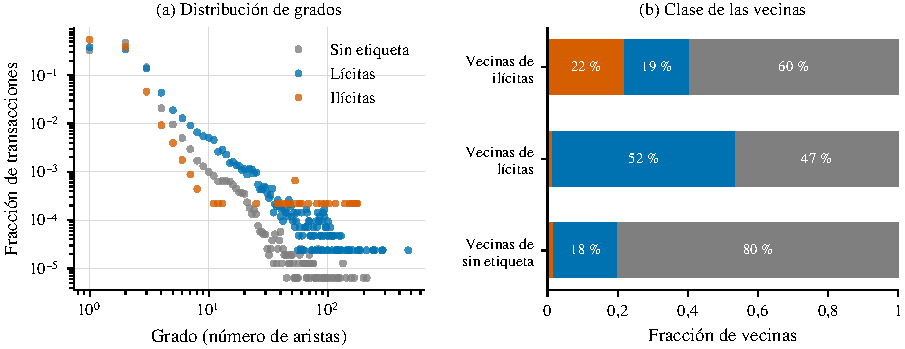
\includegraphics[width=\textwidth]{eda_grafo}
\caption{(a) Distribución del número de aristas por transacción según su clase, en escala
logarítmica. (b) Clase de las vecinas de las transacciones de cada clase, contando cada arista
desde sus dos extremos.}
\label{fig:eda}
\end{figure}

La homofilia de aristas entre transacciones etiquetadas es alta, 0,954, pero está dominada por
las aristas entre lícitas, que son la gran mayoría. La composición de las vecinas de las
ilícitas cuenta otra historia (Figura \ref{fig:eda}b): solo el 21,8~\% de las vecinas de una
transacción ilícita es ilícita, el 18,5~\% es lícita y el 59,6~\% no tiene etiqueta. Visto por
transacción, el 70~\% de las ilícitas no tiene ninguna vecina ilícita. En la tarea de esta tesis,
en la que las transacciones sin etiqueta cuentan como negativas, una ilícita está rodeada sobre
todo de negativas. La señal del fraude, por tanto, está principalmente en las variables de la
propia transacción, y una arquitectura que la promedia con sus vecinas sin darle un peso propio
la diluye (Sección \ref{sec:propiedades}). Este rasgo anticipa el bajo rendimiento de GCN.

\section{Partición temporal y exclusión del cierre del mercado}\label{sec:particion}

La partición respeta el orden del tiempo: el modelo se entrena con los pasos más antiguos y
se evalúa con los más recientes, de modo que nunca ve el futuro. La partición habitual en la
literatura usa los pasos 1 a 34 para entrenar y los pasos 35 a 49 para evaluar, y en este
trabajo se dividió esa evaluación en validación (35 a 42) y prueba (43 a 49).

En el paso 43 se cerró un mercado ilegal importante, y los autores de Elliptic reportaron que
desde ese momento ningún modelo detectaba las nuevas transacciones ilícitas
\cite{Weber2019Elliptic}. Es un cambio en la distribución de los datos a lo largo del tiempo
\cite{Gama2014Drift}: lo que el modelo aprendió de los mercados que existían deja de describir
la actividad ilícita posterior. Con la partición habitual, la prueba completa cae después del
cierre. En la corrida de esta tesis con esa partición, el mejor modelo de cada arquitectura
obtuvo en prueba un PR-AUC entre 0,005 y 0,012, frente a 0,006 que obtendría un clasificador
al azar (Anexo \ref{anx:original}).

Por ello el estudio principal usa solo los pasos 1 a 42 y los reparte en tres bloques
contiguos: entrenamiento con los pasos 1 a 29, validación con los pasos 30 a 35 y prueba con
los pasos 36 a 42 (Figura \ref{fig:particion} y Tabla \ref{tab:particion}). Los pasos 43 a 49
no se usan.

\begin{figure}[ht]
\centering
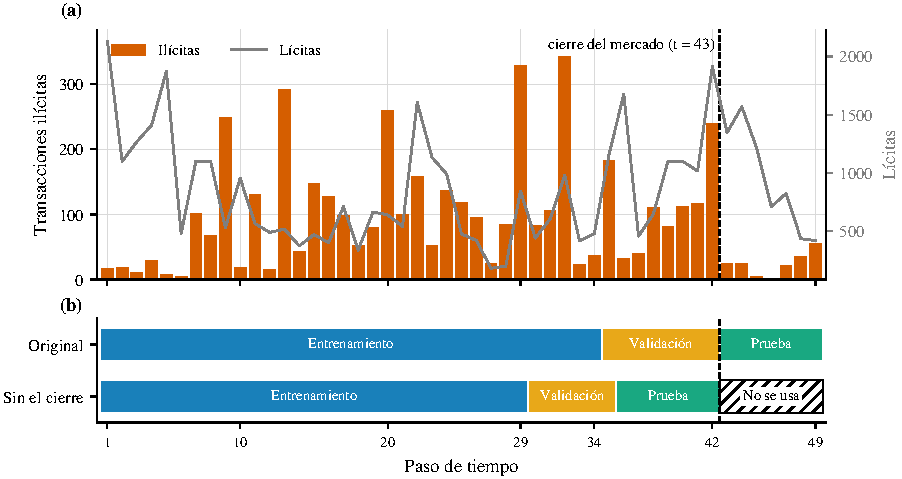
\includegraphics[width=\textwidth]{particion_temporal}
\caption{(a) Transacciones ilícitas (barras) y lícitas (línea) por paso de tiempo en Elliptic.
La línea discontinua marca el cierre del mercado ilegal en el paso 43. (b) Partición original
y partición sin el cierre usada en el estudio principal; en esta última los pasos 43 a 49 no
se usan.}
\label{fig:particion}
\end{figure}

\begin{table}[ht]
\centering
\caption{Transacciones por parte de cada partición. Negativas son lícitas más sin etiqueta;
la razón es negativas por cada ilícita.}
\label{tab:particion}
\small
% Generado por tesis_v4/scripts/analisis.py. No editar a mano.
\begin{tabular}{llrrrr}
\toprule
Partición & Parte & Pasos & Ilícitas & Negativas & Razón \\
\midrule
Original & Entrenamiento & 1 a 34 & 3.462 & 132.803 & 1:38{,}4 \\
 & Validación & 35 a 42 & 914 & 36.906 & 1:40{,}4 \\
 & Prueba & 43 a 49 & 169 & 29.515 & 1:174{,}6 \\
\midrule
Sin el cierre & Entrenamiento & 1 a 29 & 2.871 & 117.933 & 1:41{,}1 \\
 & Validación & 30 a 35 & 773 & 20.195 & 1:26{,}1 \\
 & Prueba & 36 a 42 & 732 & 31.581 & 1:43{,}1 \\
\bottomrule
\end{tabular}

\end{table}

La partición tiene tres costos que conviene declarar. Primero, el entrenamiento dispone de
2.871 transacciones ilícitas en lugar de 3.462, es decir, 591 menos que con la partición
habitual. Segundo, los cortes en los pasos 29 y 35 los escogieron los autores para que
validación y prueba tuvieran cada una cerca de una sexta parte de las ilícitas anteriores al
cierre; no responden a un criterio externo. Tercero, la prueba ya no mide la capacidad del
modelo para adaptarse a un cambio drástico del mercado, sino su desempeño en un periodo
posterior al entrenamiento pero en condiciones parecidas. Esta tesis no estudia la adaptación
a ese cambio, sino la estabilidad de las explicaciones, y para ello necesita modelos que
detecten de verdad.

\section{Escenarios de desbalance}\label{sec:escenarios}

El nivel de desbalance se modifica solo en el entrenamiento; validación y prueba conservan
siempre su proporción real. Los escenarios principales protegen la señal del fraude: no quitan
transacciones ilícitas, sino que submuestrean las negativas o sobremuestrean las ilícitas. Las
negativas se submuestrean de forma estratificada, conservando la misma mezcla de lícitas y sin
etiqueta que en el escenario nativo, con una semilla de datos fija (2026) que es distinta de la
semilla del modelo. Submuestrear significa sacar transacciones de la función de pérdida, no
del grafo: las transacciones descartadas siguen transmitiendo información a sus vecinas.

\begin{itemize}
  \item \textbf{Nativo (1:41,1).} Las 2.871 ilícitas y las 117.933 negativas del entrenamiento.
  \item \textbf{1:10 y 1:20.} Las 2.871 ilícitas y 28.710 o 57.420 negativas.
  \item \textbf{1:10 con SMOTE.} Las 2.871 ilícitas, 2.871 ilícitas sintéticas y 57.420
        negativas. Cada sintética interpola los atributos de una ilícita y de una de sus
        vecinas más cercanas en el espacio de atributos \cite{Chawla2002SMOTE}, se añade al
        grafo en el mismo paso de tiempo y hereda las aristas de la ilícita de la que parte.
  \item \textbf{1:100 y 1:200.} Escenarios de estrés solicitados por el director para forzar el
        desbalance más allá del real. Como el nativo ya usa todas las negativas, la única forma
        de llegar a esas razones es quitar ilícitas: se conservan 1.179 y 589 ilícitas, con
        las 117.933 negativas.
\end{itemize}

Los escenarios de estrés cambian dos cosas a la vez, la proporción y la cantidad absoluta de
ejemplos ilícitos, por lo que sus resultados se analizan junto a los principales pero se
interpretan con esa salvedad.

\section{Modelos y entrenamiento}\label{sec:entrenamiento}

Se entrenan cuatro arquitecturas de GNN para clasificar nodos: GCN \cite{Kipf2017GCN},
GraphSAGE \cite{Hamilton2017GraphSAGE}, GAT \cite{Velickovic2018GAT} y TAGCN
\cite{Du2017TAGCN}, descritas en la Sección \ref{sec:gnn}. Todas reciben el grafo completo y
producen una probabilidad de que cada transacción sea ilícita.

\textbf{Compensación del desbalance.} Se comparan tres funciones de pérdida (Sección
\ref{sec:desbalance}): entropía cruzada sin ajuste; entropía cruzada con pesos por clase
inversamente proporcionales a su frecuencia en el entrenamiento, de modo que cada clase aporta
la mitad de la pérdida total; y \textit{focal loss} \cite{Lin2020Focal} con $\gamma = 2$ y
$\alpha = 0{,}75$ como peso de la clase ilícita.

\textbf{Búsqueda de hiperparámetros.} Para cada combinación de arquitectura, escenario y
pérdida se hace una búsqueda bayesiana de 8 ensayos que maximiza el PR-AUC de validación.
El primer ensayo usa valores tomados de la literatura y los siguientes se proponen con un
estimador de Parzen. Cada ensayo entrena hasta 50 épocas, con parada temprana a las 10 épocas
sin mejora. El espacio es el mismo para las cuatro arquitecturas: dimensión oculta en
$\{64, 128, 148\}$, 2 o 3 capas, \textit{dropout} entre 0,1 y 0,5, tasa de aprendizaje entre
$10^{-4}$ y $10^{-2}$ y decaimiento de pesos entre $10^{-5}$ y $10^{-3}$, las dos últimas en
escala logarítmica. GAT busca además 2 o 4 cabezas de atención y TAGCN un orden de filtro $K$
entre 2 y 4. Por memoria, GAT se limita a 2 capas: con 148 dimensiones y 8 cabezas el
grafo completo no cabe en una GPU de 8~GB. Todas las arquitecturas reciben el mismo número de
ensayos y de épocas, para que la comparación no confunda arquitectura con presupuesto de
cómputo.

\textbf{Entrenamiento final y semillas.} Con los mejores hiperparámetros se entrena el modelo
final hasta 150 épocas con Adam, con parada temprana a las 20 épocas sin mejora del F1 de
validación. Esto se repite con tres semillas de modelo (42, 43 y 44); las semillas 43 y 44
reutilizan los hiperparámetros encontrados con la 42, de modo que la diferencia entre semillas
refleja solo la aleatoriedad del entrenamiento. Los hiperparámetros elegidos se listan en el Anexo
\ref{anx:tablas}. La búsqueda prefirió para TAGCN siempre 128 dimensiones y 3 capas, con órdenes
de filtro de 2 a 4, y para GAT siempre 2 capas; GraphSAGE alternó entre 2 y 3 capas y GCN eligió
casi siempre 2. El cálculo en GPU no es determinista a nivel de
pesos, porque las sumas de mensajes usan operaciones atómicas, lo que se suma a esa
aleatoriedad.

\textbf{Evaluación del rendimiento.} La métrica principal es el PR-AUC, el área bajo la curva
de precisión y exhaustividad, porque bajo un desbalance fuerte el ROC-AUC puede ser alto
aunque el modelo produzca muchas más falsas alarmas que aciertos \cite{Saito2015PR}. Se
reporta también el ROC-AUC. El umbral de decisión se fija en la validación, como el que
maximiza el F1, sin usar información de la prueba.

\textbf{Filtro de calidad.} Explicar un modelo que no aprendió no informa sobre el problema.
Por eso cada modelo se marca como aprobado si en validación, con umbral 0,5, alcanza un F1 de
al menos 0,30 y un coeficiente de Matthews \cite{Chicco2020MCC} de al menos 0,15. El filtro se
usa para interpretar los resultados, no para excluir modelos de la medición: todos los modelos
se explican, y los análisis principales se restringen a las arquitecturas que aprenden.

\section{Explicadores}\label{sec:explicadores}

\textbf{Transacciones explicadas.} Se explican las mismas 30 transacciones para todos los
modelos: 30 ilícitas de validación sorteadas con una semilla fija (1234) entre las 773
ilícitas de los pasos 30 a 35. Usar el mismo conjunto permite comparar explicaciones entre
modelos. Se explica la validación y no la prueba porque es el periodo con el que se
seleccionó el modelo y donde su comportamiento está mejor caracterizado. Las 30 transacciones son ilícitas, pero no todas son
verdaderos positivos para cada modelo: con el umbral de 0,5, los modelos con pesos por clase
aciertan en promedio entre 16,5 (TAGCN) y 22,3 (GCN) de ellas. Se explican todas, porque la
pregunta es cuán reproducible es la explicación de una predicción, sea acertada o no, y porque
restringirse a los aciertos de cada modelo impediría comparar modelos sobre las mismas
transacciones.

\textbf{Subgrafo receptivo.} Una GNN de $L$ capas solo usa, para predecir una transacción, la
información de sus vecinas a $L$ saltos o menos (a $L \cdot K$ saltos en TAGCN). Cada
explicación se calcula sobre ese subgrafo, y se verifica que la predicción del modelo en el
subgrafo coincida con la del grafo completo. Esto reduce la memoria de varios gigabytes a
unos pocos megabytes sin cambiar lo que se explica.

Se usan cinco explicadores, descritos en la Sección \ref{sec:xai}:

\begin{itemize}
  \item \textbf{GNNExplainer} \cite{Ying2019GNNExplainer}, que optimiza una máscara sobre las
        variables de los nodos del subgrafo durante 100 iteraciones con tasa de aprendizaje
        0,01. La importancia de cada variable es la media de su máscara sobre los nodos del
        subgrafo.
  \item \textbf{PGExplainer} \cite{Luo2020PGExplainer}, que entrena una red que asigna
        importancia a las aristas. Se entrena durante 100 épocas con 50 nodos, de los cuales al
        menos 25 son ilícitos. Como explica aristas y no variables, su estabilidad se reporta
        aparte.
  \item \textbf{Shapley por muestreo} \cite{Strumbelj2014Explaining, Castro2009Polynomial},
        que estima la contribución de cada variable promediando 50 permutaciones aleatorias;
        una variable ausente toma el valor medio de esa variable en el subgrafo.
  \item \textbf{Integrated Gradients} \cite{Sundararajan2017IG}, que integra el gradiente a lo
        largo del camino recto entre una referencia y la transacción, con 100 pasos. La
        referencia es la mediana del entrenamiento, que tras el escalado es el vector cero. Es
        determinista.
  \item \textbf{Expected Gradients} \cite{Erion2021Expected}, que promedia Integrated
        Gradients sobre 200 referencias tomadas al azar de 5.000 transacciones negativas del
        entrenamiento.
\end{itemize}

Ninguno de los explicadores de variables se entrena previamente: los dos de gradiente y el de
Shapley se aplican directamente al modelo, y GNNExplainer optimiza una máscara nueva para cada
transacción. Solo PGExplainer tiene una fase de entrenamiento propia.

\textbf{Réplicas.} Cada explicador se ejecuta cinco veces sobre cada transacción y cada modelo,
con semillas distintas. La estabilidad mide cuánto se parecen esas cinco explicaciones.

\subsection*{Detalles de implementación}

Los modelos y los explicadores se implementaron con PyTorch 2.6 y PyTorch Geometric 2.7; la
búsqueda de hiperparámetros con Optuna 4.8; las métricas con scikit-learn 1.8 y las pruebas
estadísticas con SciPy 1.17. GNNExplainer y PGExplainer son las implementaciones de PyTorch
Geometric. GNNExplainer se configuró para producir una máscara por variable y por nodo
(\texttt{node\_mask\_type="attributes"}) y una máscara por arista, y explica la salida del
modelo, no la etiqueta verdadera. Dos parámetros por defecto de PGExplainer se modificaron
porque producían resultados inválidos en Elliptic: el coeficiente de tamaño de la máscara se
bajó de 0,05 a 0,005, porque con el valor por defecto la máscara colapsaba a cero en todas las
aristas, y la temperatura se fijó en 1 en lugar del esquema de 5 a 2, porque con este último
la pérdida desbordaba a valores no numéricos. Además, los 50 nodos con que se entrena
PGExplainer se toman solo entre los que reciben al menos una arista: cerca del 30~\% de los
nodos de entrenamiento no recibe ninguna, y en ellos la pérdida de PGExplainer no está definida.
Shapley por muestreo, Integrated Gradients y Expected Gradients son implementaciones propias
(\texttt{src/explainability/}).

\section{Medidas de estabilidad}\label{sec:medidas}

Sea $\mathbf{a}^{(r)} \in \mathbb{R}^{165}$ el vector de importancias que la réplica $r$
asigna a las variables de una transacción. La estabilidad de esa transacción es el promedio,
sobre los $\binom{5}{2} = 10$ pares de réplicas, de una medida de acuerdo $s$:
\begin{equation}
  E = \frac{1}{10} \sum_{r < r'} s\!\left(\mathbf{a}^{(r)}, \mathbf{a}^{(r')}\right),
\end{equation}
y la estabilidad de un modelo es el promedio de $E$ sobre las 30 transacciones. Se usan tres
medidas de acuerdo:

\begin{description}
  \item[Spearman global (principal).] La correlación de rangos de Spearman
        \cite{Spearman1904} entre los dos vectores completos de 165 importancias. Es la medida
        más usada en la literatura y permite comparar con otros trabajos.
  \item[Spearman sobre las variables distintas de cero.] La misma correlación, calculada solo
        sobre las variables cuyo valor en la transacción es distinto de cero.
  \item[Jaccard top-10.] El índice de Jaccard \cite{Jaccard1912} entre los conjuntos de las 10
        variables más importantes de cada réplica, $|A \cap B| / |A \cup B|$. Si las dos
        réplicas comparten $k$ de sus 10 variables, el índice vale $k / (20 - k)$: compartir
        3, 5 o 7 variables da 0,18, 0,33 y 0,54.
\end{description}

Las dos medidas adicionales responden a un artefacto que se detectó durante el estudio. Una
variable que vale cero recibe una importancia nula o casi nula de los cuatro explicadores de
variables, por razones distintas en cada uno: Integrated Gradients multiplica el gradiente por
la diferencia entre la variable y la referencia, que es cero; la máscara de GNNExplainer anula
las entradas sin gradiente; y en Shapley y Expected Gradients la referencia suele coincidir con
cero. Esas variables, cerca de la mitad, quedan siempre al final del orden en cualquier
réplica y en cualquier modelo, y el Spearman global cuenta su acuerdo como si fuera
información. El tamaño de ese efecto se puede calcular. Si dos explicaciones solo coinciden en
dejar empatadas al final las variables nulas de la transacción y ordenan las demás al azar, su
correlación de Spearman media sobre las 30 transacciones es 0,81 (entre 0,54 y 0,86 según la
transacción, porque la fracción de variables nulas va del 23~\% al 50~\%). Ese es el piso que la
medida principal da sin que las explicaciones compartan nada sobre las variables que sí
importan (\texttt{tesis\_v4/scripts/piso\_spearman.py}).
El Spearman sobre las variables distintas de cero elimina el bloque, y el Jaccard top-10 solo
mira las variables que el analista vería primero.

Además de la estabilidad entre réplicas de un mismo modelo, se mide el acuerdo entre las
explicaciones medias de dos modelos distintos sobre las mismas transacciones: entre semillas,
entre escenarios, entre arquitecturas y entre explicadores.

\section{Control de pesos aleatorios}\label{sec:control}

Una explicación estable no es necesariamente una explicación del modelo. Si el explicador
dependiera solo de los datos de la transacción, daría el mismo resultado con cualquier modelo.
Para comprobarlo se aplica la prueba de aleatorización de parámetros de Adebayo et al.
\cite{Adebayo2018Sanity}: para cada arquitectura y semilla, en el escenario nativo con pesos por
clase (12 modelos), se explican las mismas 30 transacciones con el modelo entrenado y con dos
redes de la misma arquitectura e hiperparámetros pero con pesos aleatorios, sin entrenar. Se
reporta el acuerdo entre la explicación del modelo entrenado y la de la red aleatoria. Si ese
acuerdo es tan alto como la estabilidad entre réplicas, el orden de las variables no depende
de lo que el modelo aprendió.

\section{Análisis estadístico}\label{sec:estadistica}

La unidad independiente es el modelo entrenado, es decir, una arquitectura con una semilla.
Los modelos de una misma semilla en distintos escenarios parten de los mismos pesos iniciales y
de los mismos hiperparámetros, y sus explicaciones resultan casi idénticas (acuerdo de 0,96
entre escenarios con la misma semilla frente a 0,92 entre semillas). Tratarlos como
observaciones independientes inflaría la significancia, por lo que las pruebas se construyen
así:

\begin{description}
  \item[H1 (escenario).] Prueba de Friedman \cite{Friedman1937} con 9 bloques (3 arquitecturas
        que aprenden por 3 semillas) y 6 tratamientos (los escenarios), con pesos por clase. Se
        complementa con una prueba de equivalencia de dos pruebas unilaterales (TOST)
        \cite{Lakens2017TOST} entre el nativo y 1:200 con margen de 0,05: rechazar ambas
        hipótesis nulas indica que la diferencia, si existe, es menor que el margen.
  \item[H2 (arquitectura).] Prueba de Friedman con 3 bloques (las semillas) y 4 tratamientos
        (las arquitecturas), sobre la media de los cuatro escenarios principales con pesos por
        clase. Con tres bloques la prueba tiene poca potencia, por lo que se reporta además en
        cuántas semillas queda primera cada arquitectura.
  \item[H3 (compensación).] Prueba de signos pareada sobre 9 pares (arquitectura por semilla,
        media de los cuatro escenarios principales), de pesos por clase frente a
        \textit{focal loss} y frente a sin ajuste.
\end{description}

Los intervalos de confianza de las figuras se obtienen por \textit{bootstrap} sobre los
modelos \cite{Efron1979Bootstrap}. Todas las pruebas se repiten con las tres medidas de
estabilidad, y una conclusión se considera sólida solo si las tres coinciden.

\chapter{Resultados}\label{cap:resultados}

Este capítulo presenta los resultados de la corrida principal, con la partición sin el cierre
del mercado. Primero se muestra que esa partición recupera una prueba informativa (Sección
\ref{sec:res_cierre}) y cómo rinden los modelos según el escenario y la pérdida (Sección
\ref{sec:res_rend}). Después se contrastan las tres hipótesis (Secciones \ref{sec:res_h1} a
\ref{sec:res_h3}) y se examina qué parte de la estabilidad medida depende del modelo (Sección
\ref{sec:res_control}). Salvo que se indique otra cosa, cada cifra es la media de tres
semillas de modelo.

\section{La partición sin el cierre recupera la prueba}\label{sec:res_cierre}

La Figura \ref{fig:cierre} compara el rendimiento en prueba de las dos particiones, en el
escenario nativo y con la pérdida que obtuvo el mayor PR-AUC de validación para cada
arquitectura. Con la partición original, cuya prueba cae después del cierre, ningún modelo
supera al azar. Sin el cierre, tres de las cuatro arquitecturas detectan: GraphSAGE alcanza un
PR-AUC de 0,273, TAGCN de 0,244 y GAT de 0,172, entre 7 y 12 veces el valor del azar (0,023).
GCN queda en 0,085. El ROC-AUC sube de valores entre 0,48 y 0,71 a valores entre 0,73 y 0,88.
El mejor modelo de toda la matriz, GraphSAGE con pesos por clase en el escenario 1:20, obtiene
en prueba un PR-AUC de 0,306 y un ROC-AUC de 0,901.

\begin{figure}[ht]
\centering
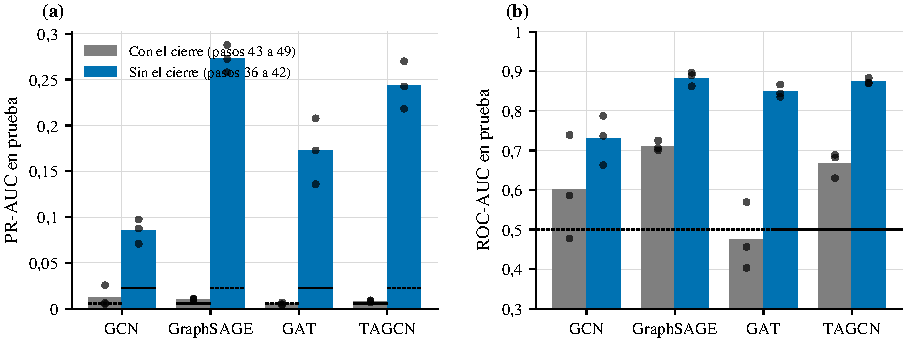
\includegraphics[width=\textwidth]{efecto_cierre}
\caption{Rendimiento en prueba con la partición original (prueba en los pasos 43 a 49,
después del cierre) y con la partición sin el cierre (prueba en los pasos 36 a 42). Escenario
nativo, pérdida elegida por validación. Las barras son la media de tres semillas, los puntos
cada semilla y las líneas discontinuas el valor del azar: la prevalencia en (a) y 0,5 en (b).}
\label{fig:cierre}
\end{figure}

La Figura \ref{fig:curvas_test} muestra las curvas completas. La curva de precisión y
exhaustividad deja ver lo que el ROC-AUC oculta: con la mitad de las ilícitas recuperadas, la precisión de GraphSAGE y de TAGCN
ronda 0,3, es decir, unas dos falsas alarmas por cada acierto. La Tabla \ref{tab:rend_nativo}
resume las cifras.

\begin{figure}[ht]
\centering
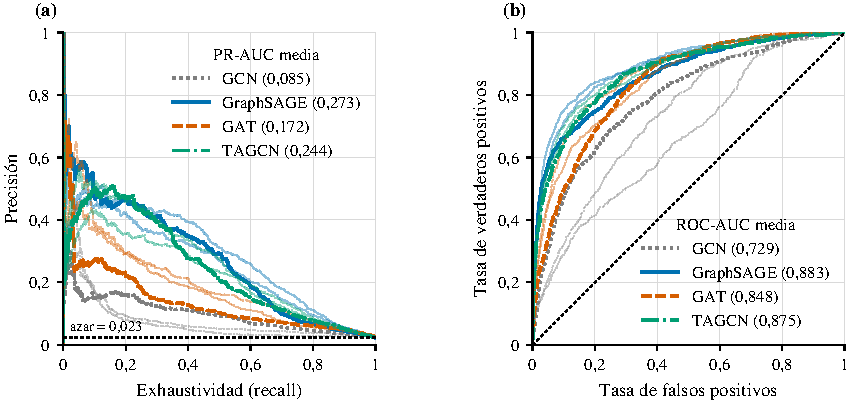
\includegraphics[width=\textwidth]{curvas_nativo_test}
\caption{Curvas de precisión y exhaustividad (a) y ROC (b) en la prueba de la partición sin el
cierre, escenario nativo, con la pérdida elegida por validación para cada arquitectura. Trazo
grueso: semilla 42; trazos finos: semillas 43 y 44. Entre paréntesis, el área media de las tres
semillas.}
\label{fig:curvas_test}
\end{figure}

\begin{table}[ht]
\centering
\caption{Rendimiento en el escenario nativo con la pérdida elegida por validación (media
$\pm$ desviación estándar de tres semillas). Filtro: modelos que superan el filtro de calidad
en validación.}
\label{tab:rend_nativo}
\small
% Generado por tesis_v4/scripts/analisis.py. No editar a mano.
\begin{tabular}{llcccc}
\toprule
Arquitectura & Pérdida elegida & PR-AUC val. & PR-AUC prueba & ROC-AUC prueba & Filtro \\
\midrule
GCN & Focal loss & 0{,}214 $\pm$ 0{,}054 & 0{,}085 $\pm$ 0{,}013 & 0{,}729 $\pm$ 0{,}063 & 0/3 \\
GraphSAGE & Focal loss & 0{,}478 $\pm$ 0{,}038 & 0{,}273 $\pm$ 0{,}015 & 0{,}883 $\pm$ 0{,}018 & 3/3 \\
GAT & Sin ajuste & 0{,}282 $\pm$ 0{,}027 & 0{,}172 $\pm$ 0{,}036 & 0{,}848 $\pm$ 0{,}016 & 2/3 \\
TAGCN & Focal loss & 0{,}529 $\pm$ 0{,}074 & 0{,}244 $\pm$ 0{,}026 & 0{,}875 $\pm$ 0{,}007 & 3/3 \\
\midrule
Azar & & 0{,}037 & 0{,}023 & 0{,}5 & \\
\bottomrule
\end{tabular}

\end{table}

\section{Rendimiento según el escenario y la pérdida}\label{sec:res_rend}

La Figura \ref{fig:perdida} y la Tabla \ref{tab:rend_esc} muestran el PR-AUC de validación de
cada combinación. Tres regularidades se observan.

\textbf{La mejor pérdida depende del escenario.} En el escenario nativo, \textit{focal loss}
iguala o supera a los pesos por clase: en GraphSAGE, 0,478 frente a 0,326; en TAGCN, 0,529
frente a 0,212. En 1:10, la entropía sin ajuste es la mejor en ambas (0,551 y 0,594). No hay
una pérdida que sea la mejor en todos los escenarios.

\textbf{Con poco fraude solo resisten los pesos por clase.} En 1:100 y 1:200, la
\textit{focal loss} de GraphSAGE cae a 0,189 y 0,054, y la de TAGCN a 0,282 y 0,054. Los pesos
por clase mantienen a GraphSAGE en 0,447 y 0,420, y a TAGCN en 0,357 y 0,307. Es el mismo
comportamiento que en la partición original.

\textbf{La entropía sin ajuste es frágil.} En GraphSAGE pasa de 0,551 en 1:10 a 0,035 en 1:20
y se queda en el nivel del azar en todos los escenarios más desbalanceados; en TAGCN baja de
0,594 a 0,046 entre 1:10 y 1:100. Cuando el desbalance supera cierto punto, el modelo minimiza
la pérdida prediciendo casi siempre la clase negativa. GAT es la excepción: es la arquitectura
en la que la entropía sin ajuste supera más veces el filtro de calidad (Tabla \ref{tab:filtro}).

\begin{figure}[ht]
\centering
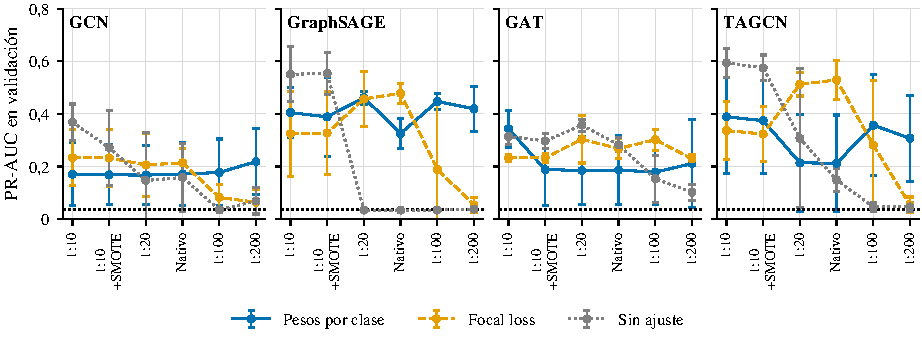
\includegraphics[width=\textwidth]{perdida_por_escenario}
\caption{PR-AUC de validación por escenario y pérdida (media y desviación estándar de tres
semillas). La línea discontinua es el valor del azar (0,037).}
\label{fig:perdida}
\end{figure}

\begin{table}[ht]
\centering
\caption{PR-AUC de validación por escenario, arquitectura y pérdida (media de tres semillas).}
\label{tab:rend_esc}
\scriptsize
\setlength{\tabcolsep}{4pt}
% Generado por tesis_v4/scripts/analisis.py. No editar a mano.
\begin{tabular}{llcccccc}
\toprule
Arquitectura & Pérdida & 1:10 & 1:10 + SMOTE & 1:20 & Nativo & 1:100 & 1:200 \\
\midrule
GCN & Pesos por clase & 0{,}171 & 0{,}169 & 0{,}167 & 0{,}171 & 0{,}177 & 0{,}219 \\
 & Focal loss & 0{,}234 & 0{,}233 & 0{,}206 & 0{,}214 & 0{,}083 & 0{,}064 \\
 & Sin ajuste & 0{,}369 & 0{,}271 & 0{,}147 & 0{,}159 & 0{,}035 & 0{,}069 \\
\midrule
GraphSAGE & Pesos por clase & 0{,}405 & 0{,}389 & 0{,}462 & 0{,}326 & 0{,}447 & 0{,}420 \\
 & Focal loss & 0{,}325 & 0{,}327 & 0{,}457 & 0{,}478 & 0{,}189 & 0{,}054 \\
 & Sin ajuste & 0{,}551 & 0{,}554 & 0{,}035 & 0{,}034 & 0{,}034 & 0{,}038 \\
\midrule
GAT & Pesos por clase & 0{,}344 & 0{,}188 & 0{,}185 & 0{,}187 & 0{,}179 & 0{,}211 \\
 & Focal loss & 0{,}233 & 0{,}233 & 0{,}304 & 0{,}268 & 0{,}302 & 0{,}229 \\
 & Sin ajuste & 0{,}314 & 0{,}297 & 0{,}357 & 0{,}282 & 0{,}154 & 0{,}102 \\
\midrule
TAGCN & Pesos por clase & 0{,}389 & 0{,}374 & 0{,}214 & 0{,}212 & 0{,}357 & 0{,}307 \\
 & Focal loss & 0{,}337 & 0{,}323 & 0{,}512 & 0{,}529 & 0{,}282 & 0{,}054 \\
 & Sin ajuste & 0{,}594 & 0{,}575 & 0{,}307 & 0{,}149 & 0{,}046 & 0{,}046 \\
\bottomrule
\end{tabular}

\end{table}

\textbf{GCN no aprende en este problema.} Ningún modelo GCN con pesos por clase supera el filtro
de calidad (Tabla \ref{tab:filtro}). GCN promedia a cada transacción con sus vecinas sin darle
un peso propio (Sección \ref{sec:gnn}), y en Elliptic la señal está sobre todo en la propia
transacción. Por eso los análisis de estabilidad por escenario y por pérdida se restringen a
GraphSAGE, GAT y TAGCN, y GCN se incluye solo en la comparación entre arquitecturas, con esa
salvedad. Hay que añadir que GAT con pesos por clase tampoco supera el filtro en ningún modelo,
aunque su PR-AUC de validación esté entre 0,18 y 0,34, muy por encima del azar: el filtro usa
el umbral fijo de 0,5, y con ese umbral su F1 queda entre 0,13 y 0,17. Se mantiene en el
análisis porque su PR-AUC muestra que sí ordena las transacciones mejor que el azar.

\begin{table}[ht]
\centering
\caption{Modelos que superan el filtro de calidad en validación (F1 $\geq$ 0,30 y MCC $\geq$
0,15 con umbral 0,5), de 18 por celda (6 escenarios por 3 semillas).}
\label{tab:filtro}
\small
% Generado por tesis_v4/scripts/analisis.py. No editar a mano.
\begin{tabular}{lccc}
\toprule
Arquitectura & Pesos por clase & Focal loss & Sin ajuste \\
\midrule
GCN & 0/18 & 3/18 & 6/18 \\
GraphSAGE & 10/18 & 11/18 & 6/18 \\
GAT & 0/18 & 8/18 & 11/18 \\
TAGCN & 8/18 & 13/18 & 7/18 \\
\bottomrule
\end{tabular}

\end{table}

\section{H1: el nivel de desbalance no cambia la estabilidad}\label{sec:res_h1}

La Figura \ref{fig:h1} y la Tabla \ref{tab:h1} muestran la estabilidad entre réplicas de cada
explicador en los seis escenarios, con pesos por clase y las tres arquitecturas que aprenden.
Con la medida principal, la estabilidad de GNNExplainer se mueve entre 0,917 (nativo) y 0,939
(1:100), la de Shapley entre 0,991 y 0,994 y la de Expected Gradients entre 0,918 y 0,934.
Integrated Gradients es determinista y vale 1 en todos los casos. No hay una tendencia a bajar
a medida que el desbalance se hace más extremo: 1:100 y 1:200 no son los escenarios menos
estables. Las dos medidas robustas confirman la ausencia de tendencia, aunque con valores más
bajos (Sección \ref{sec:res_control}).

\begin{figure}[ht]
\centering
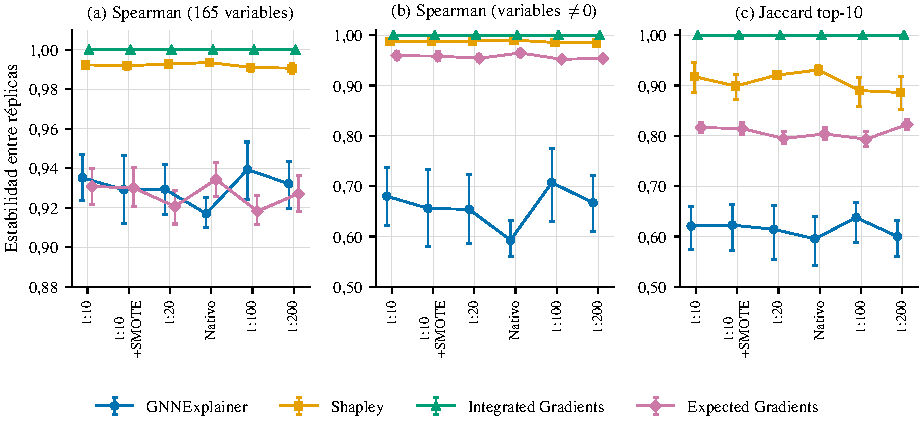
\includegraphics[width=\textwidth]{estabilidad_por_escenario}
\caption{Estabilidad entre réplicas por escenario y explicador, con las tres medidas. Pesos
por clase; media de 9 modelos (3 arquitecturas que aprenden por 3 semillas) e intervalo
\textit{bootstrap} del 95~\%.}
\label{fig:h1}
\end{figure}

\begin{table}[ht]
\centering
\caption{Estabilidad entre réplicas por escenario (pesos por clase, 9 modelos). $p$ Friedman:
igualdad de los seis escenarios. $p$ TOST: equivalencia entre nativo y 1:200 con margen 0,05
(un valor bajo indica equivalencia).}
\label{tab:h1}
\scriptsize
\setlength{\tabcolsep}{3.5pt}
% Generado por tesis_v4/scripts/analisis.py. No editar a mano.
\begin{tabular}{llcccccccc}
\toprule
Medida & Explicador & 1:10 & 1:10 + SMOTE & 1:20 & Nativo & 1:100 & 1:200 & $p$ Friedman & $p$ TOST \\
\midrule
Spearman global & GNNExplainer & 0{,}935 & 0{,}929 & 0{,}929 & 0{,}917 & 0{,}939 & 0{,}932 & 0{,}269 & $<0{,}001$ \\
 & Shapley & 0{,}992 & 0{,}992 & 0{,}993 & 0{,}994 & 0{,}991 & 0{,}991 & 0{,}534 & $<0{,}001$ \\
 & Integrated Gradients & 1{,}000 & 1{,}000 & 1{,}000 & 1{,}000 & 1{,}000 & 1{,}000 & -- & $<0{,}001$ \\
 & Expected Gradients & 0{,}931 & 0{,}930 & 0{,}921 & 0{,}934 & 0{,}918 & 0{,}927 & 0{,}248 & $<0{,}001$ \\
\midrule
Spearman $\neq 0$ & GNNExplainer & 0{,}680 & 0{,}656 & 0{,}654 & 0{,}593 & 0{,}707 & 0{,}667 & 0{,}117 & 0{,}791 \\
 & Shapley & 0{,}988 & 0{,}987 & 0{,}988 & 0{,}990 & 0{,}985 & 0{,}985 & 0{,}448 & $<0{,}001$ \\
 & Integrated Gradients & 1{,}000 & 1{,}000 & 1{,}000 & 1{,}000 & 1{,}000 & 1{,}000 & -- & $<0{,}001$ \\
 & Expected Gradients & 0{,}959 & 0{,}958 & 0{,}954 & 0{,}965 & 0{,}952 & 0{,}954 & 0{,}552 & $<0{,}001$ \\
\midrule
Jaccard top-10 & GNNExplainer & 0{,}621 & 0{,}623 & 0{,}614 & 0{,}595 & 0{,}638 & 0{,}600 & 0{,}233 & 0{,}012 \\
 & Shapley & 0{,}918 & 0{,}899 & 0{,}921 & 0{,}931 & 0{,}890 & 0{,}886 & 0{,}117 & 0{,}394 \\
 & Integrated Gradients & 1{,}000 & 1{,}000 & 1{,}000 & 1{,}000 & 1{,}000 & 1{,}000 & -- & $<0{,}001$ \\
 & Expected Gradients & 0{,}816 & 0{,}814 & 0{,}795 & 0{,}804 & 0{,}793 & 0{,}823 & 0{,}018 & $<0{,}001$ \\
\bottomrule
\end{tabular}

\end{table}

Las pruebas confirman la lectura visual. Con la medida principal, la prueba de Friedman no
rechaza la igualdad de los seis escenarios para ningún explicador ($p = 0{,}27$ en
GNNExplainer, $0{,}53$ en Shapley y $0{,}25$ en Expected Gradients), y la prueba de
equivalencia entre el nativo y 1:200 la acepta en los tres ($p \leq 0{,}0002$): la diferencia
entre el escenario real y el más extremo es menor que 0,05. Con las medidas robustas hay dos
excepciones que conviene examinar. Con el Jaccard top-10, Friedman rechaza la igualdad en
Expected Gradients ($p = 0{,}018$), pero la diferencia entre el mejor y el peor escenario es de
0,03 y el escenario más estable es precisamente 1:200; no hay degradación. Con el Spearman sobre
las variables distintas de cero, GNNExplainer no alcanza la equivalencia ($p = 0{,}79$): sus
valores van de 0,593 (nativo) a 0,707 (1:100), con un intervalo amplio, pero de nuevo el
escenario menos estable es el nativo y no los más desbalanceados.

\textbf{Veredicto sobre H1.} La hipótesis no se sostiene. En ninguno de los cuatro explicadores
ni con ninguna de las tres medidas la estabilidad disminuye a medida que el desbalance se hace
más extremo, ni siquiera en 1:100 y 1:200, donde además se quitaron transacciones ilícitas del
entrenamiento. El mismo resultado se obtuvo con la partición original (Anexo
\ref{anx:original}).

\section{H2: no hay un orden estable entre arquitecturas}\label{sec:res_h2}

\begin{figure}[ht]
\centering
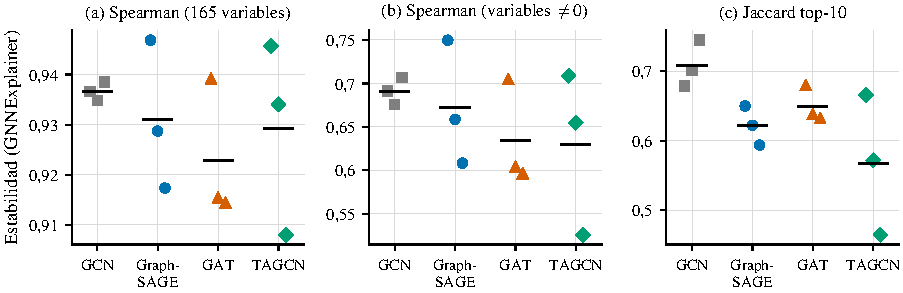
\includegraphics[width=\textwidth]{estabilidad_por_arquitectura}
\caption{Estabilidad de GNNExplainer por arquitectura con las tres medidas (pesos por clase,
media de los cuatro escenarios principales). Cada punto es una semilla; la línea horizontal es
la media.}
\label{fig:h2}
\end{figure}

\begin{table}[ht]
\centering
\caption{Estabilidad por arquitectura (pesos por clase, media de los escenarios principales,
3 semillas). $p$ (4): Friedman con las cuatro arquitecturas; $p$ (3): sin GCN. Primera: número
de semillas en que cada arquitectura obtiene el mayor valor.}
\label{tab:h2}
\scriptsize
\setlength{\tabcolsep}{3.5pt}
% Generado por tesis_v4/scripts/analisis.py. No editar a mano.
\begin{tabular}{llccccccl}
\toprule
Medida & Explicador & GCN & GraphSAGE & GAT & TAGCN & $p$ (4) & $p$ (3) & Primera \\
\midrule
Spearman global & GNNExplainer & 0{,}937 & 0{,}931 & 0{,}923 & 0{,}929 & 0{,}532 & 0{,}264 & GCN 2, GraphSAGE 1 \\
 & Shapley & 0{,}996 & 0{,}994 & 0{,}994 & 0{,}991 & 0{,}042 & 0{,}097 & GCN 3 \\
 & Expected Gradients & 0{,}923 & 0{,}935 & 0{,}932 & 0{,}920 & 0{,}172 & 0{,}097 & GraphSAGE 2, GAT 1 \\
\midrule
Spearman $\neq 0$ & GNNExplainer & 0{,}691 & 0{,}672 & 0{,}635 & 0{,}630 & 0{,}334 & 0{,}097 & GCN 2, GraphSAGE 1 \\
 & Shapley & 0{,}993 & 0{,}991 & 0{,}990 & 0{,}985 & 0{,}042 & 0{,}097 & GCN 3 \\
 & Expected Gradients & 0{,}958 & 0{,}965 & 0{,}960 & 0{,}952 & 0{,}457 & 0{,}264 & GAT 1, GraphSAGE 1, GCN 1 \\
\midrule
Jaccard top-10 & GNNExplainer & 0{,}708 & 0{,}622 & 0{,}650 & 0{,}568 & 0{,}060 & 0{,}097 & GCN 2, GAT 1 \\
 & Shapley & 0{,}948 & 0{,}929 & 0{,}927 & 0{,}896 & 0{,}122 & 0{,}264 & GCN 2, GraphSAGE 1 \\
 & Expected Gradients & 0{,}798 & 0{,}800 & 0{,}816 & 0{,}806 & 0{,}532 & 0{,}264 & GAT 2, GCN 1 \\
\bottomrule
\end{tabular}

\end{table}

Con GNNExplainer, las cuatro arquitecturas quedan dentro de dos centésimas con la medida
principal (de 0,923 en GAT a 0,937 en GCN), y las semillas de una misma arquitectura se
dispersan tanto como las arquitecturas entre sí (Figura \ref{fig:h2}). Ninguna prueba de
Friedman rechaza la igualdad con GNNExplainer ($p$ entre 0,06 y 0,53) ni con Expected
Gradients, y sin GCN ninguna lo hace con ningún explicador ni medida ($p \geq 0{,}097$). La
única diferencia significativa aparece con Shapley y las cuatro arquitecturas ($p = 0{,}042$):
GCN es la más estable en las tres semillas, pero la diferencia con la última es de cinco
milésimas (0,996 frente a 0,991). Con tres semillas como bloques la prueba tiene poca potencia,
por lo que la ausencia de diferencias no prueba la igualdad; lo que sí muestra es que no hay un
orden que se repita.

Un resultado llama la atención: GCN, la arquitectura que no aprende, obtiene las explicaciones
más estables con GNNExplainer en dos de las tres semillas y en las tres medidas. Esto anticipa
lo que muestra la Sección \ref{sec:res_control}: una explicación estable no es necesariamente
una explicación de algo aprendido.

\textbf{Veredicto sobre H2.} La hipótesis no se sostiene entre las arquitecturas que aprenden:
GraphSAGE, GAT y TAGCN producen explicaciones con estabilidad indistinguible. En la partición
original GraphSAGE había resultado la más estable en las tres semillas; ese orden no se repite
sin el cierre, y por tanto no se puede afirmar.

\section{H3: la técnica de compensación no cambia la estabilidad}\label{sec:res_h3}

\begin{table}[ht]
\centering
\caption{Estabilidad por técnica de compensación (3 arquitecturas que aprenden, media de los
escenarios principales). PC $>$ FL y PC $>$ SA: en cuántos de los 9 pares de arquitectura y
semilla pesos por clase supera a \textit{focal loss} o a sin ajuste, con el $p$ de la prueba
de signos.}
\label{tab:h3}
\scriptsize
\setlength{\tabcolsep}{3.5pt}
% Generado por tesis_v4/scripts/analisis.py. No editar a mano.
\begin{tabular}{llccccc}
\toprule
Medida & Explicador & Pesos por clase & Focal loss & Sin ajuste & PC $>$ FL & PC $>$ SA \\
\midrule
Spearman global & GNNExplainer & 0{,}928 & 0{,}922 & 0{,}930 & 6.0/9 (0{,}508) & 4.0/9 (1{,}000) \\
 & Shapley & 0{,}993 & 0{,}995 & 0{,}994 & 0.0/9 (0{,}004) & 5.0/9 (1{,}000) \\
 & Expected Gradients & 0{,}929 & 0{,}933 & 0{,}938 & 2.0/9 (0{,}180) & 1.0/9 (0{,}039) \\
\midrule
Spearman $\neq 0$ & GNNExplainer & 0{,}646 & 0{,}626 & 0{,}668 & 5.0/9 (1{,}000) & 2.0/9 (0{,}180) \\
 & Shapley & 0{,}988 & 0{,}992 & 0{,}990 & 1.0/9 (0{,}039) & 4.0/9 (1{,}000) \\
 & Expected Gradients & 0{,}959 & 0{,}960 & 0{,}962 & 4.0/9 (1{,}000) & 4.0/9 (1{,}000) \\
\midrule
Jaccard top-10 & GNNExplainer & 0{,}613 & 0{,}598 & 0{,}625 & 5.0/9 (1{,}000) & 5.0/9 (1{,}000) \\
 & Shapley & 0{,}917 & 0{,}941 & 0{,}922 & 2.0/9 (0{,}180) & 5.0/9 (1{,}000) \\
 & Expected Gradients & 0{,}807 & 0{,}799 & 0{,}805 & 7.0/9 (0{,}180) & 4.0/9 (1{,}000) \\
\bottomrule
\end{tabular}

\end{table}

Con GNNExplainer, ninguna comparación es significativa con ninguna medida: pesos por clase
supera a \textit{focal loss} en 6 de los 9 pares con la medida principal ($p = 0{,}51$) y a
la entropía sin ajuste en 4 ($p = 1$), y las diferencias medias son menores que 0,025 con las
tres medidas. Con Shapley y Expected Gradients aparecen diferencias sistemáticas pero
minúsculas: con Shapley, \textit{focal loss} es más estable que pesos por clase en los 9 pares
($p = 0{,}004$), por dos milésimas; con Expected Gradients, la entropía sin ajuste supera a
pesos por clase en 8 de 9 ($p = 0{,}039$), por nueve milésimas. El sentido de la diferencia
cambia según el explicador, y en la corrida original con GNNExplainer era el contrario (Anexo
\ref{anx:original}).

\textbf{Veredicto sobre H3.} La hipótesis se sostiene en términos prácticos: la técnica de
compensación cambia mucho el rendimiento (Sección \ref{sec:res_rend}) pero mueve la estabilidad
de los explicadores de variables en milésimas o pocas centésimas, sin un sentido constante.

\begin{table}[ht]
\centering
\caption{Estabilidad de PGExplainer sobre las aristas del subgrafo: Spearman entre réplicas y
Jaccard de las 20 aristas principales (escenarios principales, media de 3 semillas).}
\label{tab:pg}
\small
% Generado por tesis_v4/scripts/analisis.py. No editar a mano.
\begin{tabular}{lcccccc}
\toprule
 & \multicolumn{2}{c}{Pesos por clase} & \multicolumn{2}{c}{Focal loss} & \multicolumn{2}{c}{Sin ajuste} \\
\cmidrule(lr){2-3}\cmidrule(lr){4-5}\cmidrule(lr){6-7}
Arquitectura & Spearman & Jaccard & Spearman & Jaccard & Spearman & Jaccard \\
\midrule
GCN & 0{,}517 & 0{,}630 & 0{,}325 & 0{,}645 & 0{,}322 & 0{,}608 \\
GraphSAGE & 0{,}251 & 0{,}560 & 0{,}064 & 0{,}628 & 0{,}381 & 0{,}658 \\
GAT & 0{,}305 & 0{,}621 & 0{,}514 & 0{,}625 & 0{,}458 & 0{,}675 \\
TAGCN & 0{,}504 & 0{,}769 & 0{,}121 & 0{,}628 & 0{,}288 & 0{,}650 \\
\bottomrule
\end{tabular}

\end{table}

\textbf{PGExplainer.} PGExplainer explica aristas y no variables, por lo que se analiza aparte
(Tabla \ref{tab:pg}). El grafo de Elliptic es muy disperso: la mediana de aristas en el
subgrafo receptivo de las transacciones explicadas es de 2 o 3, y la estabilidad solo se pudo
medir, en promedio, en 13 de las 30 transacciones (las demás tienen menos aristas de las
necesarias para comparar órdenes). Con tan pocas aristas, el Spearman entre réplicas es una
medida muy gruesa y el Jaccard de las 20 principales compara casi siempre conjuntos que
incluyen todas las aristas disponibles. Aun así, el Spearman va de 0,06 a 0,52 según la
combinación, sin patrón por arquitectura ni por pérdida. La conclusión es que, en este
problema, PGExplainer no produce una explicación de aristas evaluable, y que la variación entre
pérdidas no puede atribuirse a la técnica de compensación.

\section{Qué parte de la estabilidad depende del modelo}\label{sec:res_control}

Las secciones anteriores muestran que la estabilidad apenas cambia con el escenario, la
arquitectura o la pérdida. Hay dos explicaciones posibles: que los modelos aprendan casi lo
mismo en todas las condiciones, o que la estabilidad medida no dependa de lo aprendido. El
control de pesos aleatorios (Sección \ref{sec:control}) permite distinguirlas (Figura
\ref{fig:control} y Tabla \ref{tab:control}).

\begin{figure}[ht]
\centering
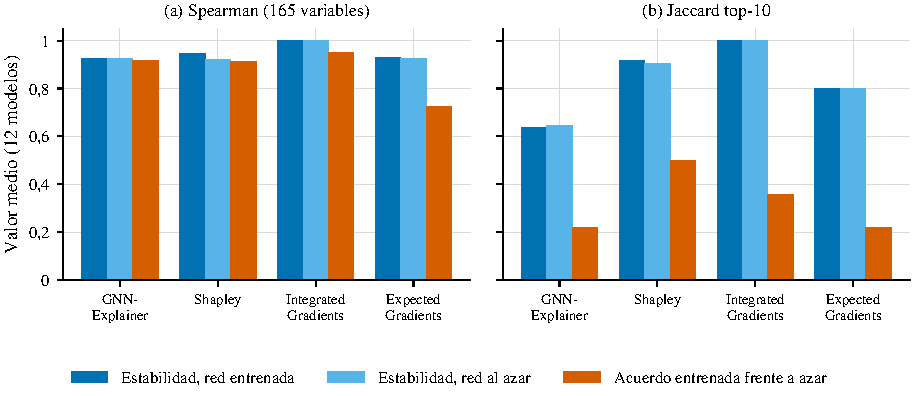
\includegraphics[width=\textwidth]{control_pesos_azar}
\caption{Control de pesos aleatorios en el escenario nativo con pesos por clase (12 modelos:
4 arquitecturas por 3 semillas). Para cada explicador, la estabilidad entre réplicas con la red
entrenada y con una red de pesos aleatorios, y el acuerdo entre la explicación de la red
entrenada y la de la red aleatoria.}
\label{fig:control}
\end{figure}

\begin{table}[ht]
\centering
\caption{Control de pesos aleatorios (media de 12 modelos).}
\label{tab:control}
\scriptsize
\setlength{\tabcolsep}{4pt}
% Generado por tesis_v4/scripts/analisis.py. No editar a mano.
\begin{tabular}{lcccccc}
\toprule
 & \multicolumn{3}{c}{Spearman global} & \multicolumn{3}{c}{Jaccard top-10} \\
\cmidrule(lr){2-4}\cmidrule(lr){5-7}
Explicador & Estab. entrenada & Estab. azar & Entrenada vs azar & Estab. entrenada & Estab. azar & Entrenada vs azar \\
\midrule
GNNExplainer & 0{,}924 & 0{,}927 & 0{,}917 & 0{,}636 & 0{,}646 & 0{,}220 \\
Shapley & 0{,}948 & 0{,}920 & 0{,}914 & 0{,}915 & 0{,}904 & 0{,}498 \\
Integrated Gradients & 1{,}000 & 1{,}000 & 0{,}950 & 1{,}000 & 1{,}000 & 0{,}357 \\
Expected Gradients & 0{,}932 & 0{,}924 & 0{,}724 & 0{,}801 & 0{,}799 & 0{,}220 \\
\bottomrule
\end{tabular}

\end{table}

\textbf{Con la medida principal, la explicación no depende del modelo.} La explicación de
GNNExplainer sobre el modelo entrenado coincide con la de una red sin entrenar con un Spearman
de 0,917, prácticamente lo mismo que coinciden dos réplicas sobre el mismo modelo (0,924). Lo
mismo ocurre con Shapley (0,914 frente a 0,948) e Integrated Gradients (0,950). Una red con
pesos aleatorios, que no aprendió nada, recibe además explicaciones igual de estables que la
entrenada (0,927 en GNNExplainer). El orden de Integrated Gradients coincide con el orden de
las variables por su valor absoluto con un Spearman de 0,97. La medida principal está dominada
por el bloque de variables en cero (Sección \ref{sec:medidas}), que ocupa las mismas posiciones
del orden con cualquier red.

\textbf{Con el Jaccard top-10, sí depende.} Las 10 variables principales de la red entrenada y
de la aleatoria comparten en promedio un índice de 0,22 con GNNExplainer y Expected Gradients,
0,36 con Integrated Gradients y 0,50 con Shapley, muy por debajo de la estabilidad entre
réplicas (0,64, 0,80, 1 y 0,92). Las variables que el analista vería primero sí cambian con los
pesos del modelo. Expected Gradients es el único explicador cuyo acuerdo con la red aleatoria
también es claramente menor que su estabilidad con la medida principal (0,724 frente a 0,932),
porque sus referencias no son el vector cero y su atribución no se anula en las variables nulas.

\textbf{Modelos igual de buenos dan explicaciones distintas.} El acuerdo entre explicaciones de
modelos distintos refuerza esta lectura. Con GNNExplainer y pesos por clase, dos semillas de la
misma arquitectura y el mismo escenario coinciden con un Spearman global de 0,929, pero con un
Jaccard top-10 de solo 0,30: comparten unas 5 de sus 10 variables principales. Cambiar de
escenario manteniendo la semilla mueve menos la explicación (Jaccard 0,60) que cambiar de
semilla manteniendo el escenario. La principal fuente de variación de la explicación no es el
desbalance, sino la aleatoriedad del entrenamiento.

\textbf{Los explicadores no coinciden entre sí.} Sobre el mismo modelo, los cuatro explicadores
de variables señalan conjuntos de variables principales muy distintos (Figura
\ref{fig:explicadores}): con el Jaccard top-10 el acuerdo va de 0,10 (GNNExplainer frente a
Shapley) a 0,49 (Integrated frente a Expected Gradients). El alto Spearman global entre
GNNExplainer e Integrated Gradients (0,84) desaparece con el Jaccard top-10 (0,29), lo que
indica que su parecido se debe sobre todo al bloque de variables nulas.

\begin{figure}[ht]
\centering
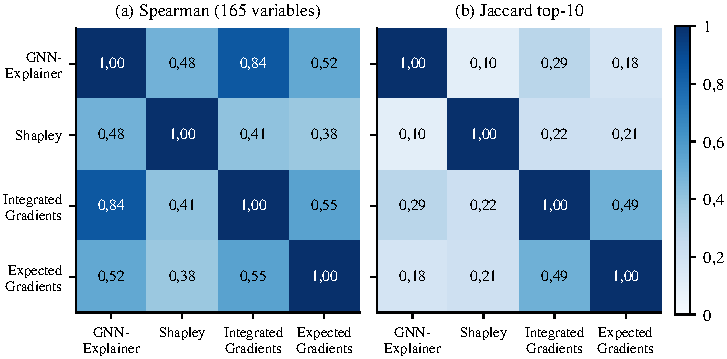
\includegraphics[width=\textwidth]{acuerdo_explicadores}
\caption{Acuerdo entre explicadores sobre el mismo modelo (GraphSAGE, GAT y TAGCN; escenarios
principales; todas las pérdidas y semillas), con el Spearman global (a) y el Jaccard top-10 (b).}
\label{fig:explicadores}
\end{figure}

\section{Síntesis}\label{sec:res_sintesis}

La Tabla \ref{tab:veredictos} resume el contraste de las hipótesis.

\begin{table}[ht]
\centering
\caption{Veredicto de las hipótesis con la partición sin el cierre.}
\label{tab:veredictos}
\small
\begin{tabularx}{\textwidth}{p{0.3\textwidth}Xp{0.2\textwidth}}
\toprule
Hipótesis & Resultado & Veredicto \\
\midrule
H1: la estabilidad baja con el desbalance & Sin tendencia en 4 explicadores y 3 medidas;
equivalencia entre nativo y 1:200 con la medida principal & No se sostiene \\
H2: la estabilidad depende de la arquitectura & Sin orden repetido entre GraphSAGE, GAT y
TAGCN; GCN, que no aprende, es la más estable & No se sostiene \\
H3: la compensación no cambia la estabilidad & Diferencias de milésimas o pocas centésimas,
con sentido que cambia según el explicador & Se sostiene en términos prácticos \\
\bottomrule
\end{tabularx}
\end{table}

Los tres veredictos tienen una lectura común que el control de pesos aleatorios aclara: con la
medida principal, la estabilidad refleja sobre todo la estructura de los datos de entrada y el
explicador, no lo que el modelo aprendió, y por eso apenas responde a los factores del diseño.
Las 10 variables principales, en cambio, sí dependen del modelo, y varían más entre semillas
que entre escenarios.

\chapter{Discusión}\label{cap:discusion}

\textbf{[Por redactar después del Capítulo \ref{cap:resultados}.]}

\chapter{Conclusiones}\label{cap:conclusiones}

\textbf{[Por redactar después del Capítulo \ref{cap:resultados}.]}


\clearpage
\phantomsection
\addcontentsline{toc}{chapter}{Referencias}
\printbibliography[title={Referencias}]

\appendix
\chapter{Corrida con la partición original}\label{anx:original}

Antes de excluir el periodo del cierre del mercado se ejecutó el estudio completo con la
partición habitual de Elliptic: entrenamiento con los pasos 1 a 34 (3.462 ilícitas y 132.803
negativas, razón 1:38,4), validación con los pasos 35 a 42 y prueba con los pasos 43 a 49. Se
entrenaron 252 modelos: las mismas 4 arquitecturas, 3 pérdidas y 3 semillas, con los escenarios
nativo, 1:10, 1:20, 1:10 con SMOTE, 1:1 (que se apartó del análisis principal), 1:100 y 1:200.
En esta partición los escenarios de estrés conservan 1.328 y 664 ilícitas. Este anexo resume
lo que esa corrida muestra y por qué motivó el cambio de partición. Los resultados completos
están en \texttt{results\_v4/}.

\section{La prueba cae al nivel del azar}

En la prueba, después del cierre, la prevalencia de ilícitas es de 0,6~\%, que es el PR-AUC
de un clasificador al azar. Con la pérdida elegida en validación, en el escenario nativo, el
PR-AUC de prueba fue de 0,010 para GraphSAGE, 0,008 para TAGCN, 0,005 para GAT y 0,012 para
GCN. El ROC-AUC fue 0,711, 0,667, 0,476 y 0,601. Ningún modelo detecta las transacciones
ilícitas posteriores al cierre, lo que reproduce lo reportado por los autores del conjunto de
datos \cite{Weber2019Elliptic}. En validación, en cambio, los modelos sí aprendían: GraphSAGE
con pesos por clase alcanzaba un PR-AUC de 0,462 frente a 0,037 del azar.

\section{Lo que se mantiene en las dos particiones}

La estabilidad de las explicaciones se mide en validación, por lo que no depende de la prueba,
y sus conclusiones generales se repiten en las dos corridas:

\begin{itemize}
  \item El nivel de desbalance no cambia la estabilidad. Con GNNExplainer, pesos por clase y
        las tres arquitecturas que aprenden, el Spearman global fue 0,946, 0,947, 0,946 y
        0,947 en 1:10, 1:10 con SMOTE, 1:20 y nativo, y 0,940 y 0,938 en 1:100 y 1:200. La
        prueba de Friedman sobre los seis escenarios no rechazó la igualdad ($p = 0{,}84$).
  \item GCN es la arquitectura más débil en las dos particiones.
  \item Con poco fraude (1:100 y 1:200) solo los pesos por clase mantienen la detección.
  \item El control de pesos aleatorios dio, sobre 12 modelos, un acuerdo entre la explicación
        del modelo entrenado y la de la red sin entrenar de 0,896 con GNNExplainer, 0,911 con
        Shapley, 0,956 con Integrated Gradients y 0,688 con Expected Gradients, frente a una
        estabilidad entre réplicas de 0,949, 0,970, 1 y 0,929.
\end{itemize}

\section{Lo que cambia}

Tres resultados de la corrida original no se repiten sin el cierre, y por eso no se presentan
como conclusiones de la tesis:

\begin{itemize}
  \item Con la partición original, GraphSAGE fue la arquitectura más estable con GNNExplainer
        en las tres semillas (Spearman global 0,964 frente a 0,939 de GAT y 0,937 de TAGCN). Sin
        el cierre ese orden desaparece (Sección \ref{sec:res_h2}).
  \item Con la partición original, pesos por clase dio explicaciones de GNNExplainer más
        estables que \textit{focal loss} en los 9 pares de arquitectura y semilla (prueba de
        signos, $p = 0{,}004$), pero con Shapley el sentido se invertía. Sin el cierre la
        diferencia con GNNExplainer tampoco se sostiene (Sección \ref{sec:res_h3}).
  \item En validación, pesos por clase era la mejor pérdida en el escenario nativo. Sin el
        cierre, \textit{focal loss} la iguala o la supera en ese escenario.
\end{itemize}

Una advertencia metodológica surgió de esta corrida y se aplica a toda la tesis: los modelos de
una misma semilla en distintos escenarios son casi idénticos, por lo que una prueba que trata
cada combinación de semilla y escenario como un bloque independiente (12 bloques) está
pseudorreplicada y exagera la significancia. Las pruebas del Capítulo \ref{cap:resultados} usan
como unidad el modelo.

\chapter{Eje sintético}\label{anx:sintetico}

Elliptic no publica el significado de sus variables ni anota qué patrón de lavado sigue cada
transacción ilícita, de modo que sobre él solo se puede medir la estabilidad de las
explicaciones, no si señalan lo correcto. Para observar esa segunda propiedad se construyó un
grafo sintético de transacciones en el que cada transacción ilícita pertenece a una tipología
conocida y en el que se sabe qué aristas y qué variables la delatan. Este anexo resume sus
resultados como evidencia complementaria; no forma parte del contraste de hipótesis.

\section{Diseño}

El generador (\texttt{phase1/synthetic\_aml\_generator.py}, opción \texttt{--v4}, semilla 42)
produce un grafo con tipologías de lavado insertadas sobre un fondo de transacciones
legítimas. Se verificó que ninguna variable aislada permite separar las clases (AUC de una
sola variable entre 0,50 y 0,62) y que las cuatro arquitecturas aprenden la tipología con un
margen de al menos 0,10. Se entrenaron 144 configuraciones: las 4 arquitecturas, 4 escenarios,
3 técnicas de compensación y 3 semillas, explicadas con GNNExplainer, PGExplainer y Shapley
por muestreo.

Los escenarios del eje sintético difieren de los de Elliptic: los niveles 1:50 y 1:100 se
obtienen quitando transacciones ilícitas. Además se miden la \textbf{plausibilidad}
(coincidencia de las variables o aristas señaladas con las que de verdad definen la
tipología; para las variables, la fracción de las variables verdaderas que aparecen entre las 3
principales) y la \textbf{fidelidad} (cuánto cambia la predicción al retirar lo señalado, fid+,
o al conservar solo lo señalado, fid$-$), cada una frente a una explicación al azar del mismo
tamaño. La fidelidad se calcula sobre lo que cada explicador explica: retirando aristas en
GNNExplainer y PGExplainer, y retirando variables en Shapley. Por eso la fidelidad de
GNNExplainer y la de Shapley no son comparables entre sí; cada una solo se compara con su propio
valor al azar.

\section{Resultados}

\begin{table}[ht]
\centering
\caption{Eje sintético: estabilidad (Spearman global), plausibilidad de variables y fidelidad
(fid+; sobre aristas en GNNExplainer y sobre variables en Shapley), con su valor al azar entre
paréntesis. Medias sobre 36 configuraciones por fila.
Fuente: \texttt{results\_phase1\_v4/summary\_v4.csv}.}
\label{tab:sintetico}
\small
\begin{tabular}{llccc}
\toprule
Arquitectura & Explicador & Estabilidad & Plausibilidad de variables & Fidelidad (fid+) \\
\midrule
GCN & GNNExplainer & 0,848 & 0,296 (0,150) & 0,147 (0,030) \\
    & Shapley      & 0,984 & 0,114 (0,150) & 0,195 (0,063) \\
GraphSAGE & GNNExplainer & 0,907 & 0,404 (0,150) & 0,363 (0,048) \\
          & Shapley      & 0,953 & 0,157 (0,150) & 0,135 (0,092) \\
GAT & GNNExplainer & 0,850 & 0,244 (0,150) & 0,264 (0,054) \\
    & Shapley      & 0,959 & 0,118 (0,150) & 0,118 (0,101) \\
TAGCN & GNNExplainer & 0,957 & 0,447 (0,150) & 0,277 (0,053) \\
      & Shapley      & 0,945 & 0,159 (0,150) & 0,154 (0,083) \\
\bottomrule
\end{tabular}
\end{table}

La Tabla \ref{tab:sintetico} muestra el resultado central del eje: el explicador más estable
no es el más correcto. Shapley por muestreo es el más estable en tres de las cuatro
arquitecturas (Spearman entre 0,95 y 0,98), pero su plausibilidad de variables no supera al
azar (entre 0,11 y 0,16 frente a 0,15). GNNExplainer es menos estable, pero es el único cuya
plausibilidad de variables supera claramente al azar (entre 0,24 y 0,45). Ambos explicadores
superan a su propia línea base de fidelidad, salvo Shapley en GAT (0,118 frente a 0,101,
$p = 0{,}22$), pero esas cifras no
permiten decir cuál es más fiel, porque miden cosas distintas. La estabilidad de GNNExplainer baja con el desbalance, de 0,92 en los niveles
nativo y 1:1 a 0,86 en 1:100, mientras que la de Shapley no cambia.

Este resultado apoya una de las conclusiones del estudio principal: la estabilidad es
necesaria pero no suficiente, y debe complementarse con pruebas de que la explicación depende
del modelo.

\section{Advertencias}

\begin{itemize}
  \item La plausibilidad de aristas no es comparable entre arquitecturas. TAGCN ve 6 saltos y
        su subgrafo receptivo contiene casi todo el grafo (mediana de 9.311 nodos y 47.311
        aristas), mientras que las otras tres ven 2 saltos (unos 36 nodos y 78 aristas). La
        plausibilidad al azar vale 0,001 en TAGCN y cerca de 0,47 en las demás, y la ganancia
        aparente de TAGCN se debe a esa línea base. Por eso la tabla no la incluye.
  \item En las arquitecturas de dos saltos, la plausibilidad de aristas de los explicadores
        apenas supera al azar (entre 0,01 y 0,03), y la de PGExplainer queda por debajo.
  \item PGExplainer falló en 24 de 432 combinaciones, todas en los escenarios 1:50 y 1:100.
\end{itemize}

\chapter{Reproducibilidad}\label{anx:reproducibilidad}
\sloppy

\section{Entorno}

Los experimentos se ejecutaron en una estación con GPU NVIDIA RTX 4060 de 8~GB, con Python
3.12 y PyTorch Geometric. Las dependencias exactas están fijadas en \texttt{uv.lock}, en la raíz
del repositorio, y se instalan con \texttt{uv sync}. El conjunto de datos Elliptic se descarga
automáticamente en \texttt{data/} la primera vez.

\section{Corrida principal (sin el cierre del mercado)}

\begin{itemize}
  \item Configuración: \texttt{configs/experiment\_v4\_precierre.yaml}.
  \item Entrenamiento y explicación: \texttt{scripts/v4/run\_precierre.sh} y
        \texttt{scripts/v4/cola\_precierre.sh}. Producen 216 modelos en
        \texttt{results\_models\_v4\_precierre/} y las explicaciones en
        \texttt{results\_v4\_precierre/} y \texttt{results\_v4\_precierre\_grad/}.
  \item Curvas y métricas de rendimiento:
        \texttt{scripts/v4/reunion\_0410/curvas.py --variante precierre}.
  \item Medidas robustas y control de pesos aleatorios:
        \texttt{scripts/v4/cola\_robusta\_precierre.sh}, que ejecuta en secuencia
        \texttt{metrica\_robusta.py} y \texttt{control\_aleatorio.py} con
        \texttt{--variante precierre}.
\end{itemize}

\section{Tablas, figuras y bibliografía del manuscrito}

Las tablas y figuras se regeneran sin GPU desde los resultados guardados:

\begin{itemize}
  \item \texttt{tesis\_v4/scripts/analisis.py}: tablas \LaTeX{} y pruebas estadísticas
        (\texttt{tesis\_v4/tablas/}).
  \item \texttt{tesis\_v4/scripts/figuras.py}: figuras en PDF vectorial
        (\texttt{tesis\_v4/figuras/}).
  \item \texttt{tesis\_v4/scripts/verificar\_referencias.py}: genera
        \texttt{bibliografia.bib} consultando Crossref por DOI y rechaza todo lo que no sea un
        artículo de revista o tenga una retractación registrada. Las únicas excepciones son
        los artículos originales de los métodos y del conjunto de datos usados, listados en
        \texttt{tesis\_v4/referencias/excepciones.bib} con la URL donde se verificaron.
\end{itemize}

\section{Determinismo}

Las semillas de datos (2026), de modelo (42, 43 y 44), de selección de transacciones (1234) y de
los explicadores están fijadas. Aun así, el entrenamiento en GPU no es determinista a nivel de
pesos, porque las agregaciones de mensajes usan sumas atómicas. Repetir la corrida reproduce
las conclusiones, pero no necesariamente todos los decimales.


\end{document}
